\documentclass{scrreprt}
\setcounter{secnumdepth}{5}
\usepackage{listings}
\usepackage{enumitem}
\usepackage{underscore}
\usepackage{graphicx}
\usepackage[bookmarks=true]{hyperref}
\usepackage[utf8]{inputenc}
\usepackage[english]{babel}
\usepackage[pass,letterpaper]{geometry}
\usepackage[export]{adjustbox}
\usepackage{subcaption}
\usepackage{float}
\graphicspath{{/home/mitansh/Downloads/sefiles/images/}}
\hypersetup{
    bookmarks=false,    % show bookmarks bar?
    pdftitle={Code Testing documnet},    % title
    pdfauthor={Akul Agrawal, Sujoy Ghosh, Mitansh Jain},                     % author
    pdfsubject={TeX and LaTeX},                        % subject of the document
    pdfkeywords={TeX, LaTeX, graphics, images}, % list of keywords
    colorlinks=true,       % false: boxed links; true: colored links
    linkcolor=black,       % color of internal links
    citecolor=black,       % color of links to bibliography
    filecolor=black,        % color of file links
    urlcolor=purple,        % color of external links
    linktoc=all            % only page is linked
}                                          %
\def\myversion{1.0}
\date{}
\title{}
\begin{document}
\begin{flushright}
    \rule{16cm}{5pt}\vskip1cm
    \begin{bfseries}
        \Huge{CS-223\\CODE TESTING\\ DOCUMENT}\\
        \vspace{1.5cm}
        for\\
        \vspace{1.5cm}
        Project 7\\
        Classroom Visualisation App-1\\
        
        \vspace{1.9cm}
        \LARGE{Prepared by: }\\
        Group-12\\
        Mitansh Jain - 160101042\\
        Sujoy Ghosh - 160101073\\
        Akul Agrawal - 160101085\\
        \vspace{1.9cm}
        \today\\
    \end{bfseries}
\end{flushright}
\tableofcontents
\listoffigures
% \listoftables

\chapter{Introduction}
This document contains the complete unit testing of our app Classroom Visualisation.
Unit testing is undertaken after each module has been coded and successfully reviewed.
The code testing team in isolation has tested different units and modules of the system.
Different members of the code testing team have submitted their reports.
In short, this document is meant to equip the reader with the bugs and shortcomings in the
working of the Classroom Visualisation App.

\chapter{Team profile for black box testing}
The code testing team comprises of the following members, all of whom are undergraduates currently pursuing Bachelor of Technology at Indian Institute of Technology Guwahati, India in the Department of Computer Science and Engineering. All of the members are currently in the second year of their degree.
\begin{enumerate}
  \item Harshit Agrawal
  \item Harshit Gupta
  \item Harshit Sharma
\end{enumerate}
All members of the team are proficient in Java and have past experience in developing android applications.

\chapter{Equivalence Class Partitioning}
\section{Module Name: Login Module}
\begin{itemize}
\item[•]\textbf{Equivalence Classes}:
\begin{enumerate}
\item \textbf{Input}: Valid Email Id, Valid password\\
\textbf{Expected Output}: Directs to start session activity. Displays "Login successful".
\item \textbf{Input}: Email Id, Valid password\\
\textbf{Expected Output}: Login Failed message displayed.
\item \textbf{Input}: Valid Email Id, Invalid password\\
\textbf{Expected Output}: Login Failed message displayed.
\item \textbf{Input}: Invalid Email Id, Invalid password\\
\textbf{Expected Output}: Login Failed message displayed.
\end{enumerate}
\item[•]\textbf{Boundary Cases}: Equivalence classes here are discrete. There are no boundary cases.
\end{itemize}

\section{Module Name: Sign Up}
\begin{itemize}
\item[•]\textbf{Equivalence Classes}:
\begin{enumerate}
\item \textbf{Input}: Duplicate email Id is entered \\
\textbf{Expected Output}: Displays "Email ID already exists.
\item \textbf{Input}: If any one field is left empty\\
\textbf{Expected Output}: Account is not created. Marks the fields left empty.
\item \textbf{Input}: Password $\neq$ Confirm Password\\
\textbf{Expected Output}: Displays "Passwords do not match".
\item \textbf{Input}: Valid email ID is entered, Name is entered, passwords entered match\\
\textbf{Expected Output}: Account created successfully.
\end{enumerate}
\item[•]\textbf{Boundary Cases}: Equivalence classes here are discrete. There are no boundary cases.
\end{itemize}

\section{Module Name: Add Student}
\begin{itemize}
\item[•]\textbf{Equivalence Classes}:
\begin{enumerate}
\item \textbf{Input}: Roll No. not integer \\
\textbf{Expected Output}: Displays "Roll Number is not an integer".
\item \textbf{Input}:  Roll No. already exists in entered course ID\\
\textbf{Expected Output}: Displays "Student already exists".
\item \textbf{Input}: Roll No. already exists in other course ID\\
\textbf{Expected Output}: Adds student successfully to database.
\item \textbf{Input}: If any one field is left empty\\
\textbf{Expected Output}: Shows error on empty fields.
\item \textbf{Input}: If all fields are filled correctly and input does not belong to any of the above class.\\
\textbf{Expected Output}: Displays "Student Record created successfully".
\end{enumerate}
\item[•]\textbf{Boundary Cases}: Equivalence classes here are discrete. There are no boundary cases.
\end{itemize}

\section{Module Name: Add Images}
\begin{itemize}
\item[•]\textbf{Equivalence Classes}:
\begin{enumerate}
\item \textbf{Input}: No. of added images $<$ 15 \\
\textbf{Expected Output}: Option to return to main menu is not shown.
\item \textbf{Input}:  No. of added images $>$ 15\\
\textbf{Expected Output}: Clicking more than 15 images should not be allowed.
\end{enumerate}
\item[•]\textbf{Boundary Cases}:
\begin{enumerate}
\item \textbf{Input}: No. of added images $=$ 15 \\
\textbf{Expected Output}: Gives option to return to main screen.
\end{enumerate}
\end{itemize}

\section{Module Name: Edit Student}
\begin{itemize}
\item[•]\textbf{Equivalence Classes}:
\begin{enumerate}
\item \textbf{Input}: Roll No. not integer \\
\textbf{Expected Output}: Displays "Roll Number is not an integer".
\item \textbf{Input}:  Roll No. already exists but in other course ID\\
\textbf{Expected Output}: Displays "Student does not exists".
\item \textbf{Input}:  Roll No. doesn't exist\\
\textbf{Expected Output}:  Displays "Student does not exists".
\item \textbf{Input}: If any one field is left empty\\
\textbf{Expected Output}: Shows error on empty fields.
\item \textbf{Input}: If all fields are filled correctly and input does not belong to any of the above class.\\
\textbf{Expected Output}: Displays "Data successfully updated".
\end{enumerate}
\item[•]\textbf{Boundary Cases}: Equivalence classes here are discrete. There are no boundary cases.
\end{itemize}

\section{Module Name: View Student List}
\begin{itemize}
\item[•]\textbf{Equivalence Classes}:
\begin{enumerate}
\item \textbf{Input}: Course ID field is left empty\\
\textbf{Expected Output}: Shows error on empty field.
\item \textbf{Input}: Invalid Course ID\\
\textbf{Expected Output}: Displays "no such course Id exists".
\item \textbf{Input}:  Valid Course ID\\
\textbf{Expected Output}: Displays list of all student that were added to data base.
\end{enumerate}
\item[•]\textbf{Boundary Cases}: Equivalence classes here are discrete. There are no boundary cases.
\end{itemize}

\section{Module Name: Delete Student Record}
\begin{itemize}
\item[•]\textbf{Equivalence Classes}:
\begin{enumerate}
\item \textbf{Input}: Roll No. not an integer\\
\textbf{Expected Output}: Displays "Roll Number not an integer".
\item \textbf{Input}: Roll No. exists.\\
\textbf{Expected Output}: Displays "Roll Number deleted". Roll Number should not be visible in table of students in from view student list module. 
\end{enumerate}
\item[•]\textbf{Boundary Cases}: Equivalence classes here are discrete. There are no boundary cases.
\end{itemize}

\section{Module name: Camera Session and Face Detection}
\begin{itemize}
\item[•]\textbf{Equivalence Classes}:
\begin{enumerate}
\item \textbf{Input}: State of student $<$ 5.\\
\textbf{Expected Output}: Bounding box color: red
\item \textbf{Input}: 5 $<$ State of student $<$ 8\\
\textbf{Expected Output}: Bounding box color: blue
\item \textbf{Input}: 8 $<$ State of student\\
\textbf{Expected Output}: Bounding box color: green
\item \textbf{Input}: More than one known students(1 to 5) are standing\\
\textbf{Expected Output}: Students should be correctly identified.

\end{enumerate}
\item[•]\textbf{Boundary Cases}: 
\begin{enumerate}
\item \textbf{Input}: State of student $=$ 5.\\
\textbf{Expected Output}: Bounding box color: blue
\item \textbf{Input}: State of student $=$ 8\\
\textbf{Expected Output}: Bounding box color: green
\item \textbf{Input}: Number of known students $=$ 1\\
\textbf{Expected Output}: Student should be correctly identified.
\item \textbf{Input}: Number of known students $=$ 0\\
\textbf{Expected Output}: Nothing should be shown.
\item \textbf{Input}: Number of unknown students $=$ 1\\
\textbf{Expected Output}: Student should marked with unknown.

\end{enumerate}
\end{itemize}




\chapter{Blackbox Testing}
\section{Module Name: Login Module}
\begin{itemize}
\item[•]\textbf{Equivalence Classes}:
\begin{enumerate}
\item \textbf{Input}: Valid Email : ghosh@gmail.com, Valid password : 12345\\
\textbf{Expected Output}: Directs to start session activity. Displays "Login successful".

\begin{figure}[H]
\begin{subfigure}{0.5\textwidth}
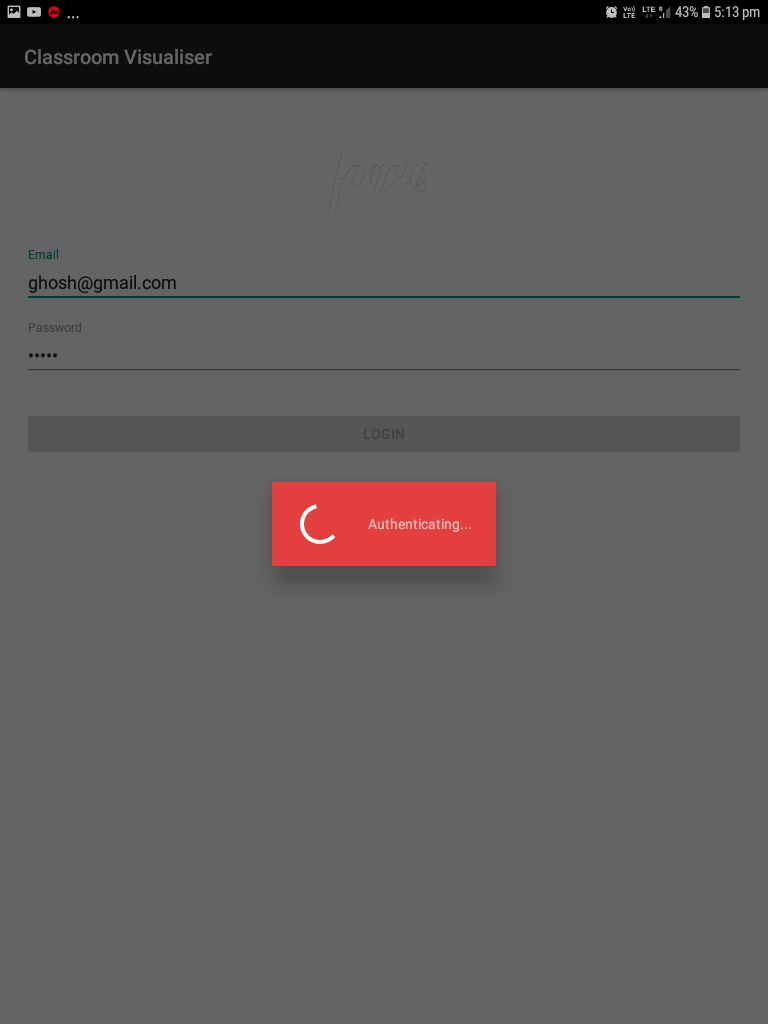
\includegraphics[width=0.85\linewidth, keepaspectratio]{logincredentials.jpg} 
\caption{Input Credentials}
\label{fig:subim1}
\end{subfigure}
\begin{subfigure}{0.5\textwidth}
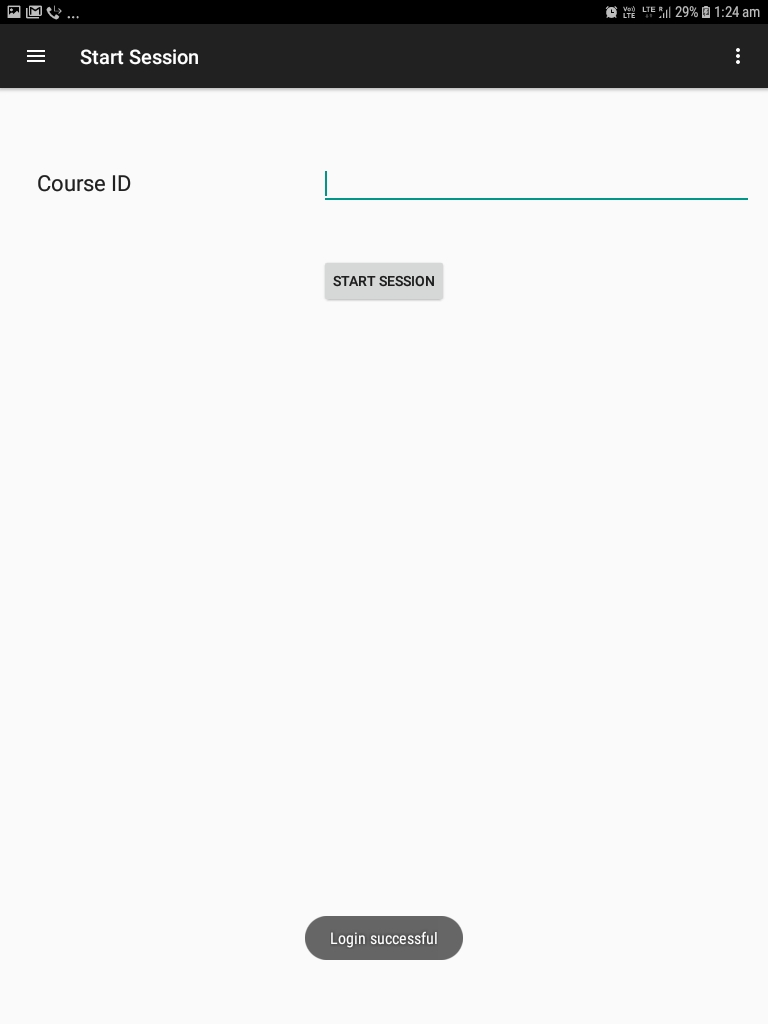
\includegraphics[width=0.85\linewidth, keepaspectratio]{logincorrect.jpg}
\caption{Output}
\label{fig:subim2}
\end{subfigure}
\end{figure}
\textbf{Output}: Directs to start session activity. Displays "Login successful". Hence we get our desired output.

\item \textbf{Input}: Invalid email : gho@gmail.com, Valid password : 12345\\
\textbf{Expected Output}: Login Failed message displayed.
\begin{figure}[H]
\centering
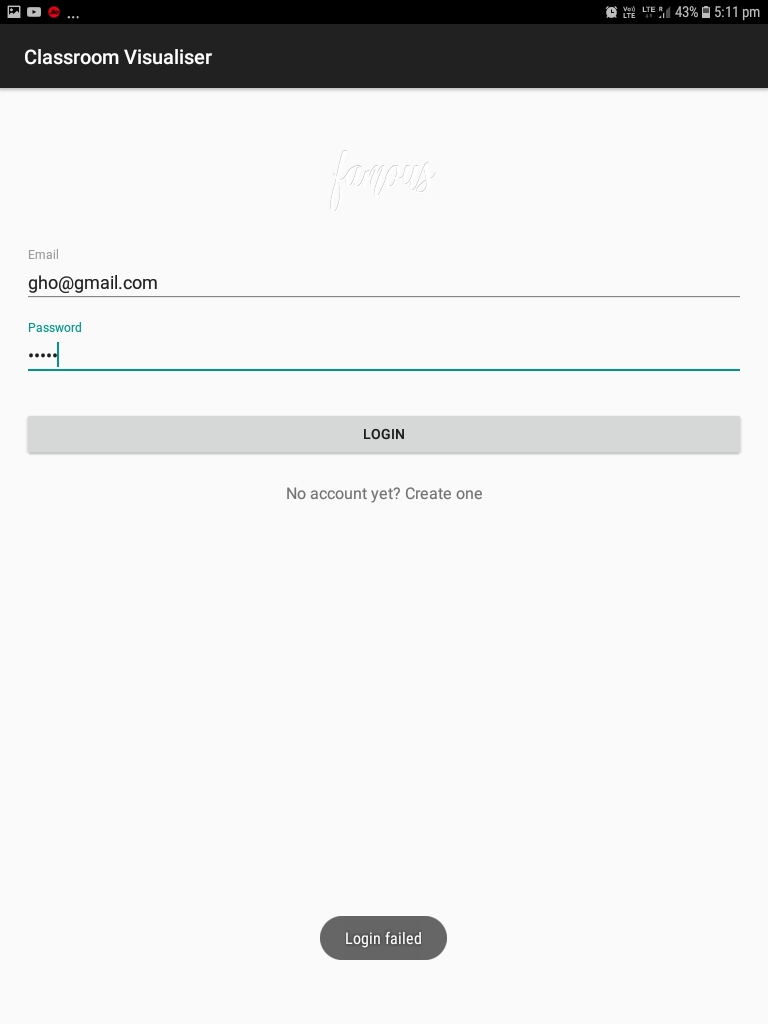
\includegraphics[width=0.42\textwidth, keepaspectratio]{loginwronguser.jpg}
\caption{Input with wrong email id}
\end{figure}
\textbf{Output}: 'Login Failed' is displayed. Hence we get our desired output.


\item \textbf{Input}: Valid Email Id : ghosh@gmail.com, Invalid password : 123456\\
\textbf{Expected Output}: Login Failed message displayed.
\begin{figure}[H]
\centering
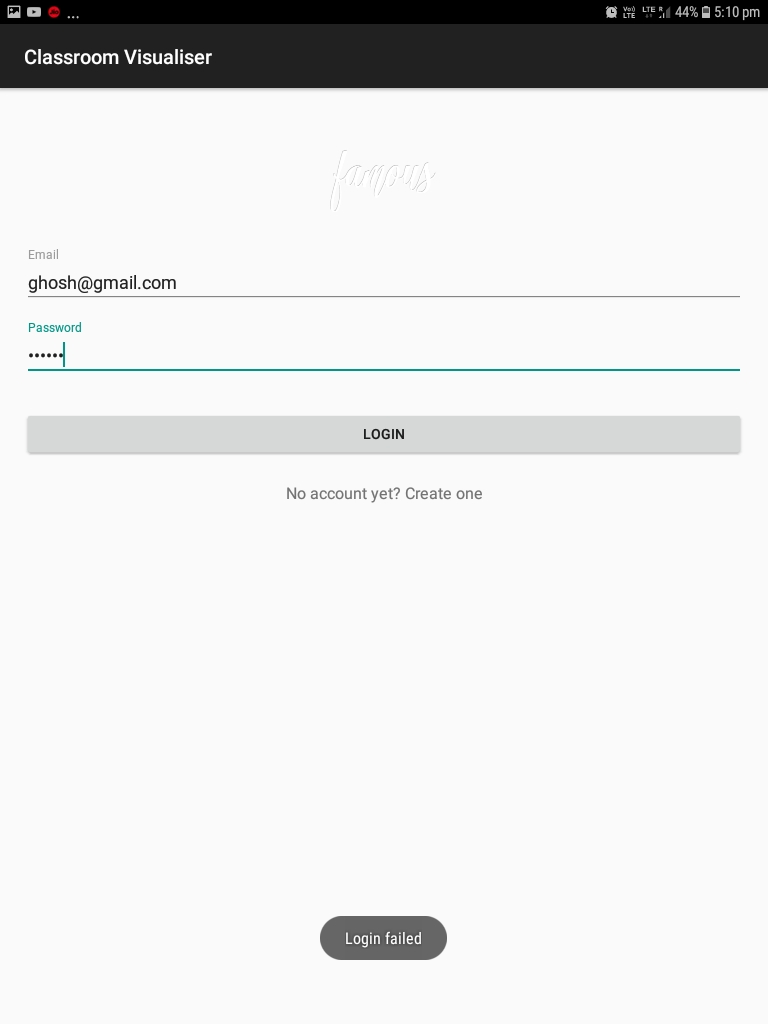
\includegraphics[width=0.42\textwidth, keepaspectratio]{loginwrongpass.jpg}
\caption{Input with wrong password}
\end{figure}
\textbf{Output}: 'Login Failed' is displayed. Hence we get our desired output.


\item \textbf{Input}: Invalid Email Id : gho@gmail.com, Invalid password : 12345678\\
\textbf{Expected Output}: Login Failed message displayed.
\begin{figure}[H]
\centering
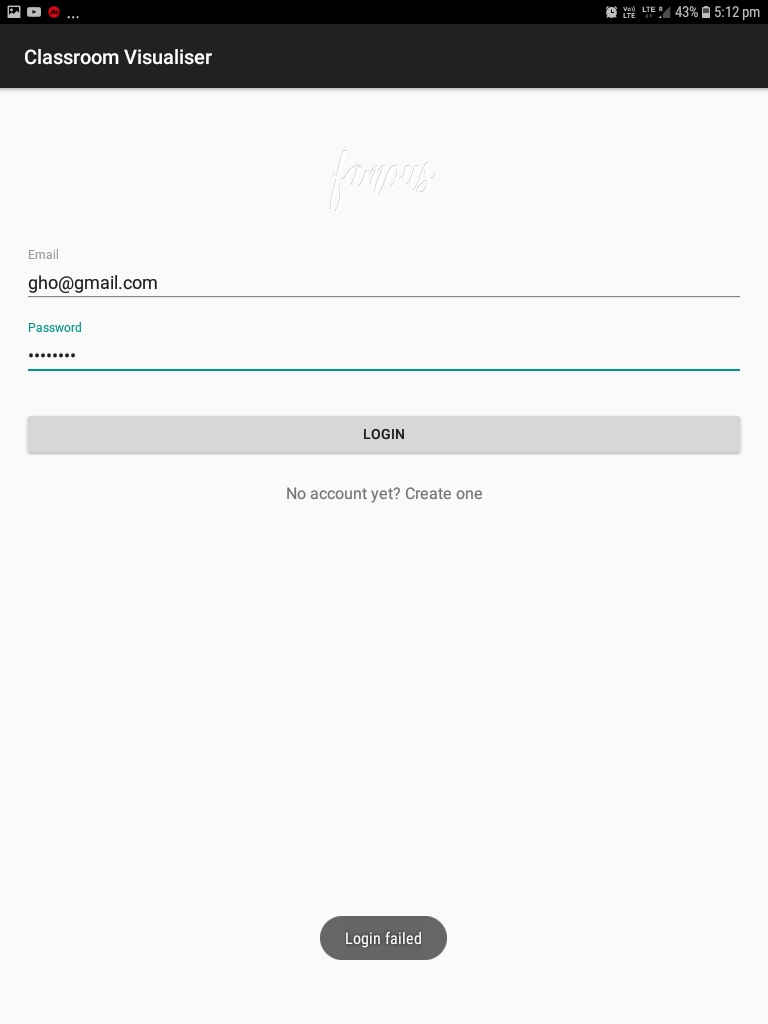
\includegraphics[width=0.42\textwidth, keepaspectratio]{loginwrongpassuser.jpg}
\caption{Input with wrong email id as well as wrong password}
\end{figure}
\textbf{Output}: 'Login Failed' is displayed. Hence we get our desired output.
\end{enumerate}
%\item[•]\textbf{Boundary Cases}: Equivalence classes here are discrete. There are no boundary cases.
\end{itemize}




\section{Module Name: Sign Up}
\begin{itemize}
\item[•]\textbf{Equivalence Classes}:
\begin{enumerate}
\item \textbf{Input}: Duplicate email Id is entered : ghosh@gmail.com \\
\textbf{Expected Output}: Displays "Email ID already exists".
\begin{figure}[H]
\begin{subfigure}{0.5\textwidth}
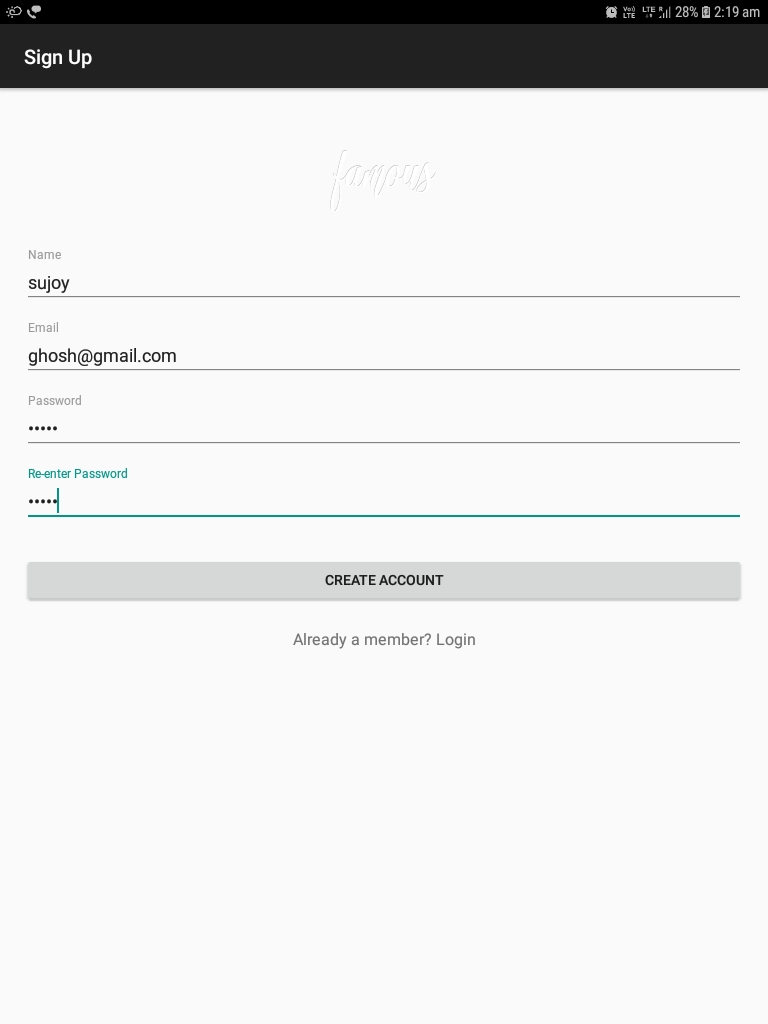
\includegraphics[width=0.85\linewidth, keepaspectratio]{signupexistemail.jpg} 
\caption{Input Credentials}
\label{fig:subim1}
\end{subfigure}
\begin{subfigure}{0.5\textwidth}
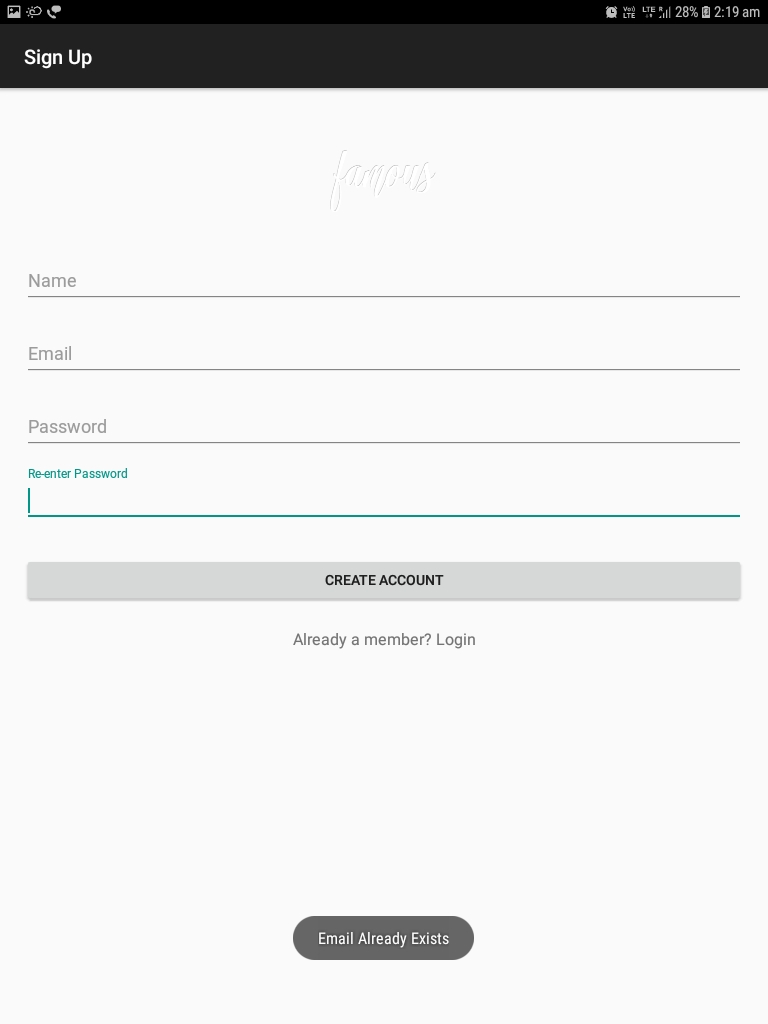
\includegraphics[width=0.85\linewidth, keepaspectratio]{signupexistemailmes.jpg}
\caption{Output : Email exists}
\label{fig:subim2}
\end{subfigure}
\end{figure}
\textbf{Output}: Displays "Email already exists". Hence we get our expected output

\item \textbf{Input}: If any one field is left empty\\
\textbf{Expected Output}: Account is not created. Marks the fields left empty.
\begin{figure}[H]
\begin{subfigure}{0.5\textwidth}
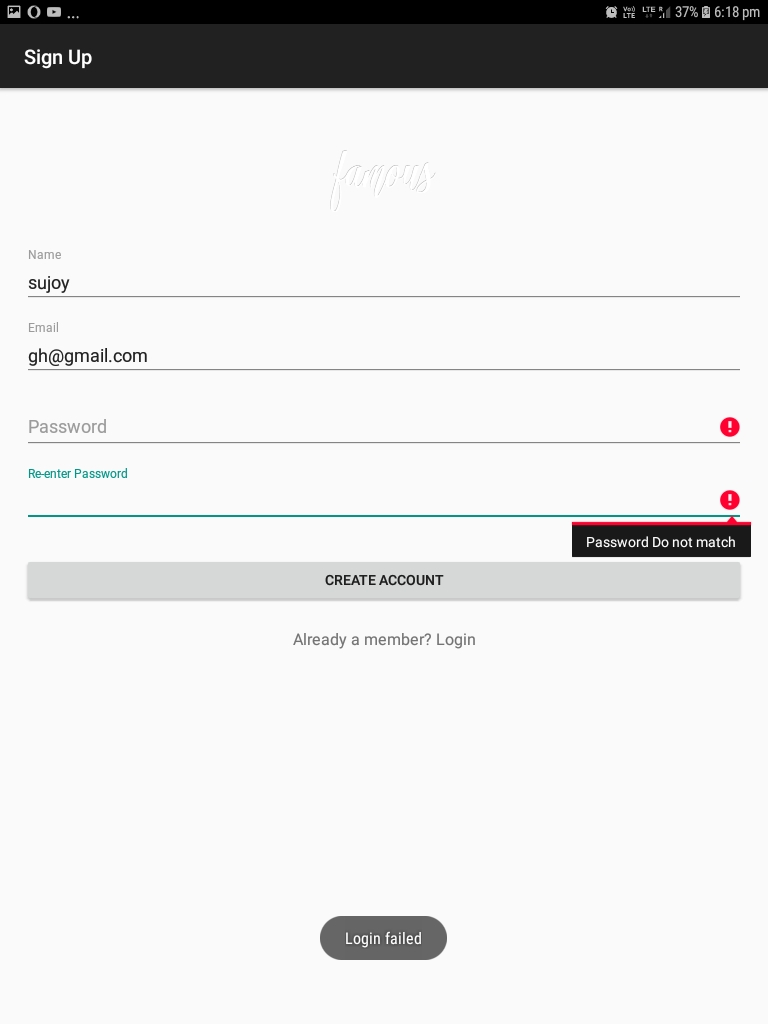
\includegraphics[width=0.85\linewidth, keepaspectratio]{signupempty.jpg} 
\caption{Input with password empty}
\label{fig:subim1}
\end{subfigure}
\begin{subfigure}{0.5\textwidth}
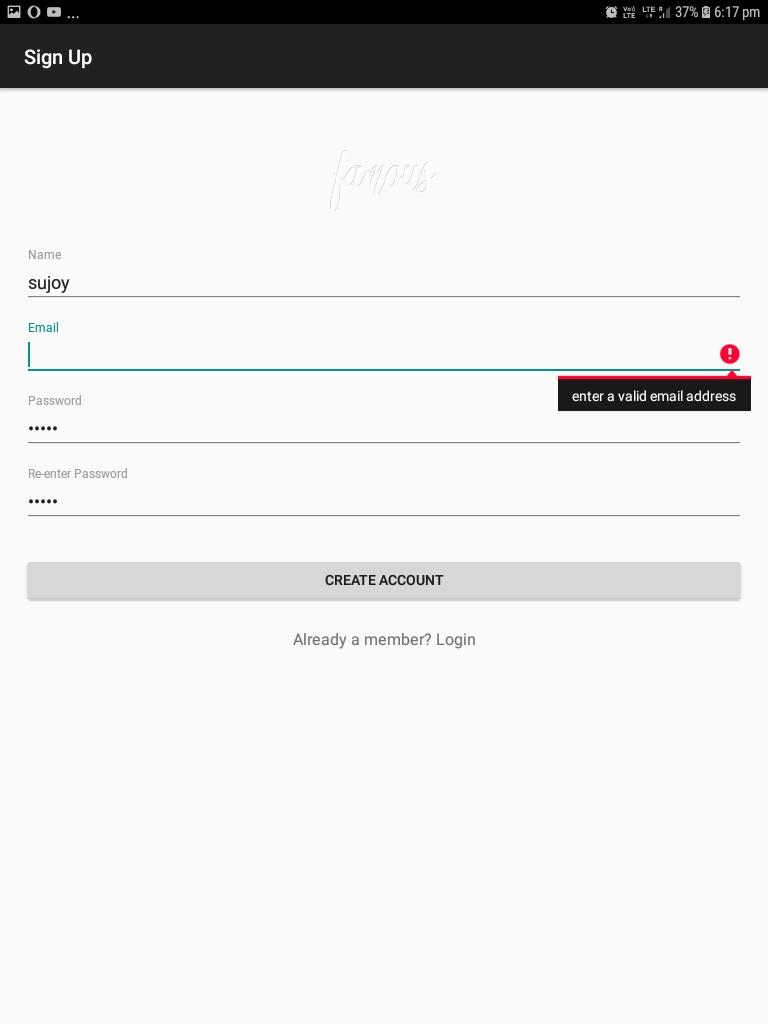
\includegraphics[width=0.85\linewidth, keepaspectratio]{signupemptyemail.jpg}
\caption{Input with email empty}
\label{fig:subim2}
\end{subfigure}
\end{figure}
\begin{figure}[H]
\begin{subfigure}{0.5\textwidth}
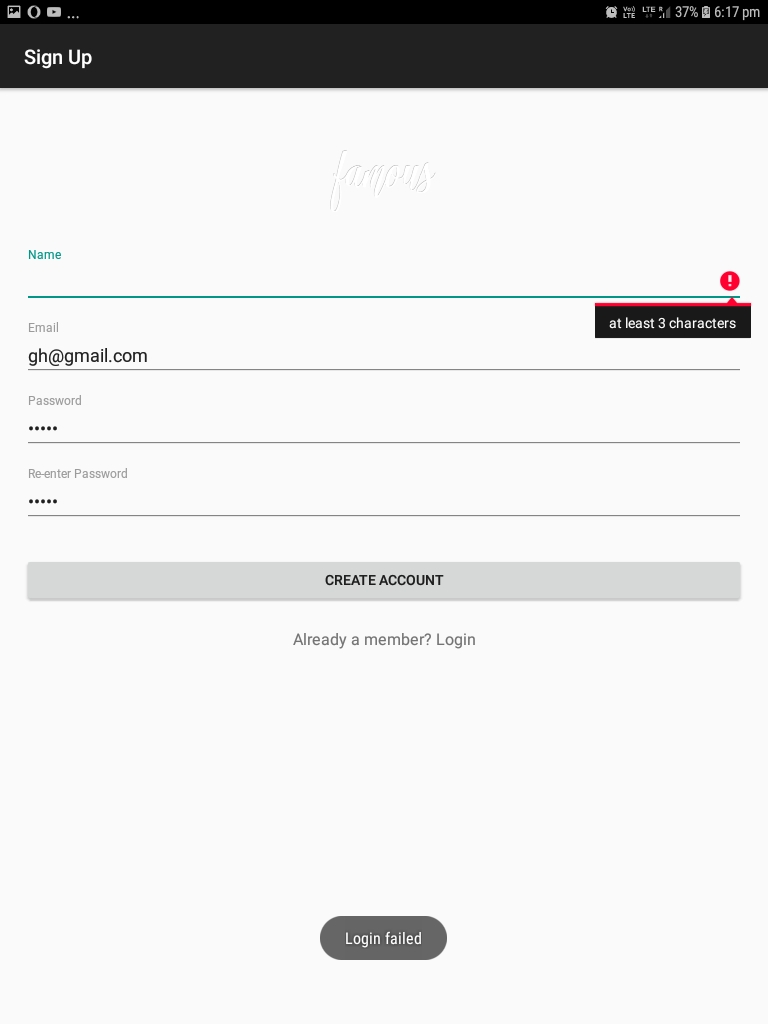
\includegraphics[width=0.85\linewidth, keepaspectratio]{signupemptyname.jpg} 
\caption{Input with name empty}
\label{fig:subim1}
\end{subfigure}
\begin{subfigure}{0.5\textwidth}
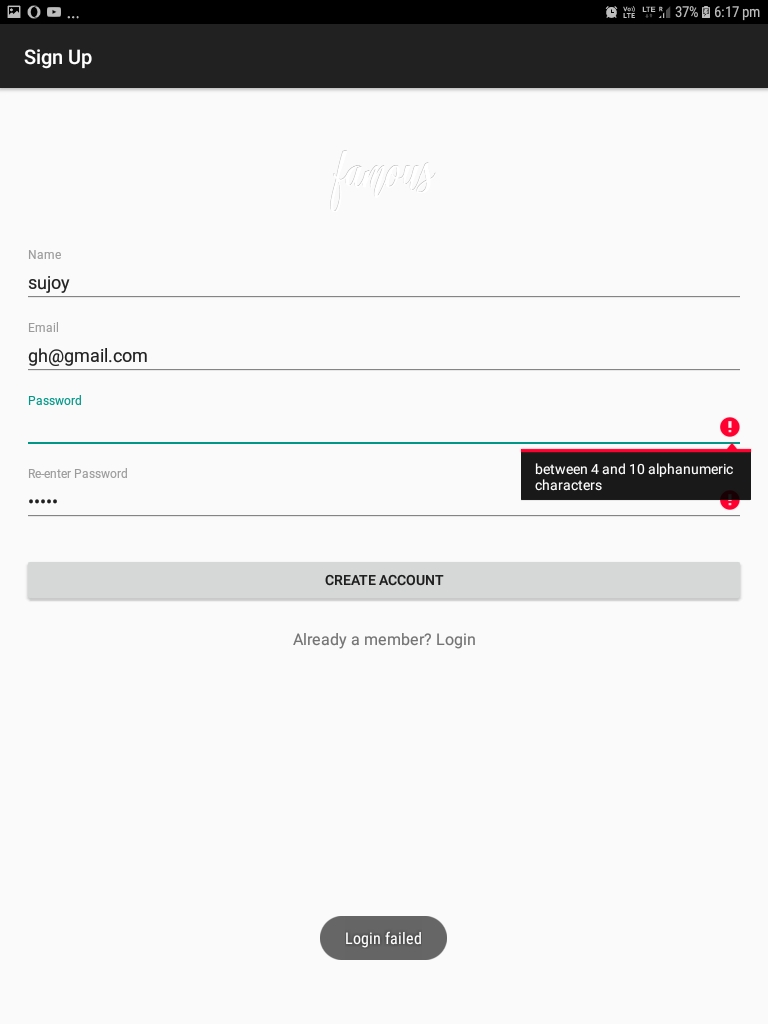
\includegraphics[width=0.85\linewidth, keepaspectratio]{signupemptypassword.jpg}
\caption{Input with password empty}
\label{fig:subim2}
\end{subfigure}
\end{figure}
\textbf{Output}: Account is not created. Hence we get our desired output.

\item \textbf{Input}: Password $\neq$ Confirm Password\\
\textbf{Expected Output}: Displays "Passwords do not match".
\begin{figure}[H]
\centering
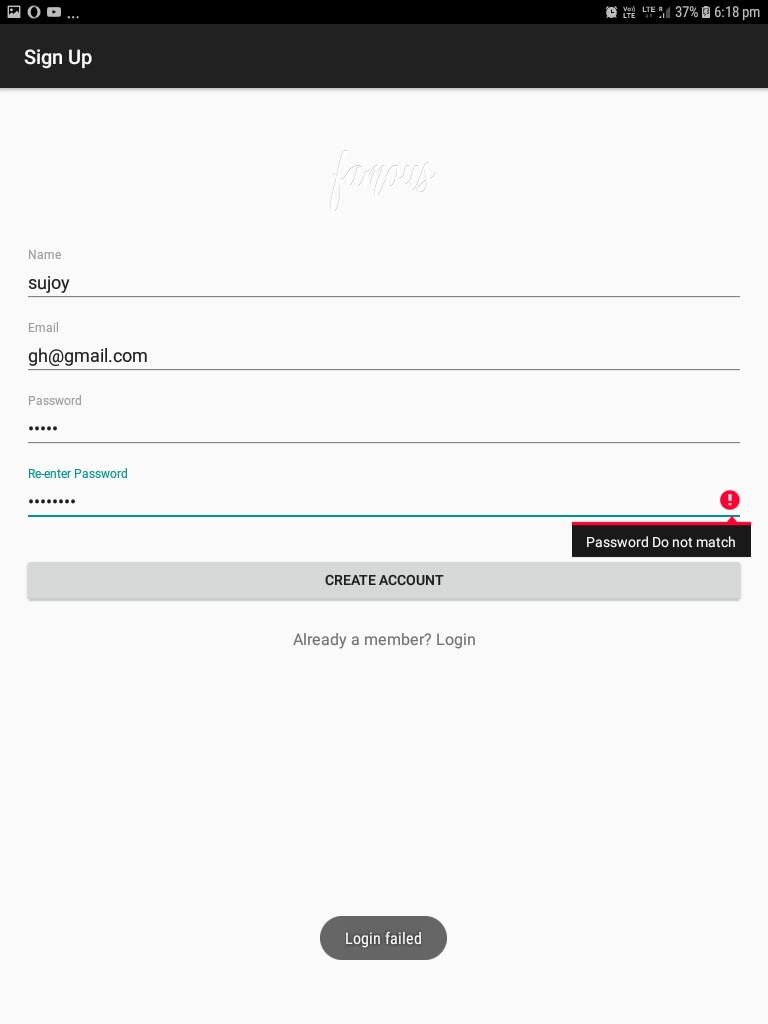
\includegraphics[width=0.42\textwidth, keepaspectratio]{signuppassnot.jpg}
\caption{Input with Password $\neq$ Confirm Password}
\end{figure}
\textbf{Output}: "Passwords do not match" is displayed. Hence we get our desired output.

\item \textbf{Input}: Valid email ID is entered, Name is entered, passwords entered match\\
\textbf{Expected Output}: Account created successfully.
\begin{figure}[H]
\begin{subfigure}{0.5\textwidth}
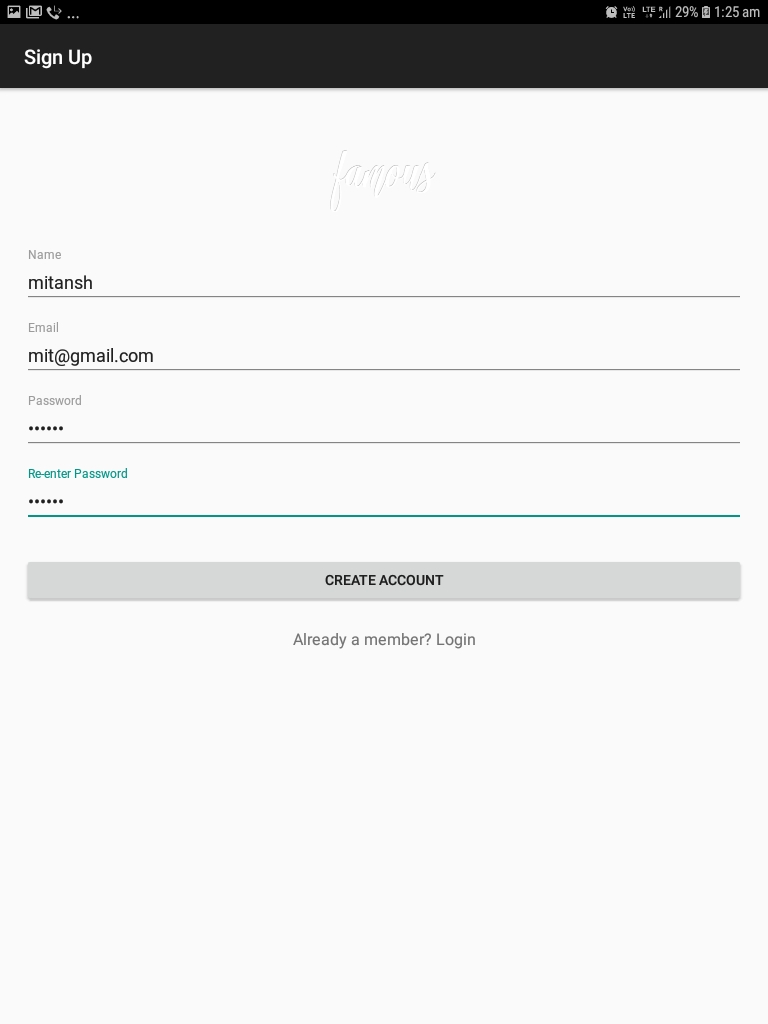
\includegraphics[width=0.85\linewidth, keepaspectratio]{signupuser.jpg} 
\caption{Input with correct credentials}
\label{fig:subim1}
\end{subfigure}
\begin{subfigure}{0.5\textwidth}
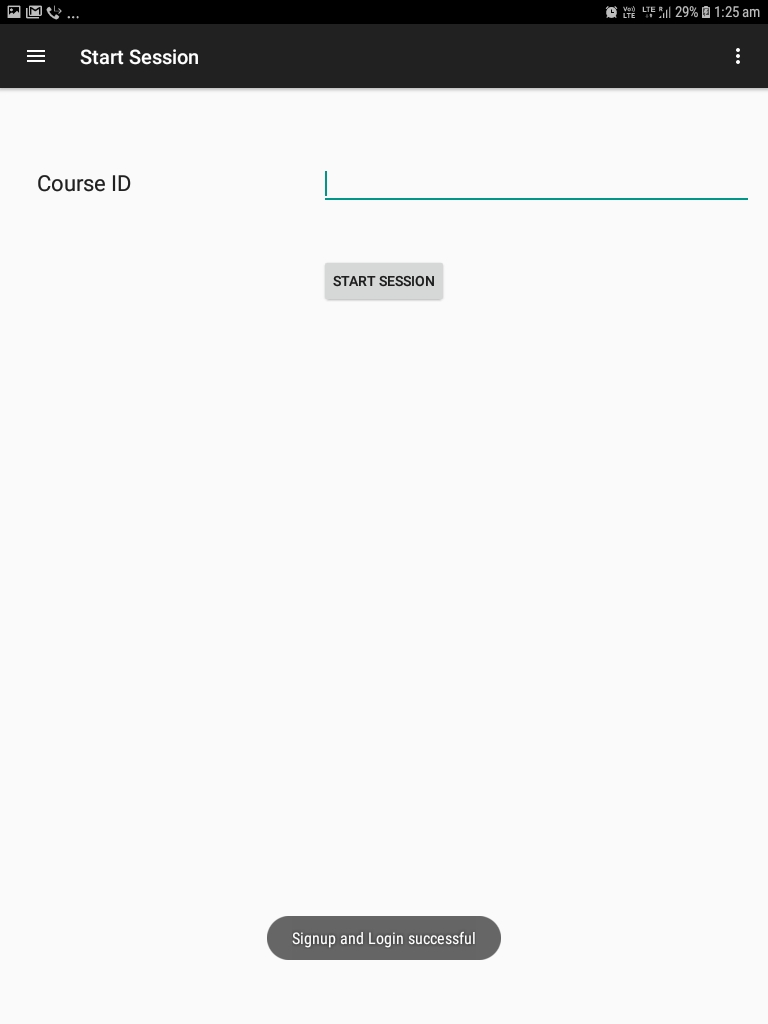
\includegraphics[width=0.85\linewidth, keepaspectratio]{signupsucc.jpg}
\caption{Output with successful login}
\label{fig:subim2}
\end{subfigure}
\caption{Successful signup}
\end{figure}
\textbf{Output}: "Signup and login successful" is displayed. Hence we get our desired output
\end{enumerate}
%\item[•]\textbf{Boundary Cases}: Equivalence classes here are discrete. There are no boundary cases.
\end{itemize}

\section{Module Name: Add Student}
\begin{itemize}
\item[•]\textbf{Equivalence Classes}:
\begin{enumerate}
\item \textbf{Input}: Roll No. not integer \\
\textbf{Expected Output}: Displays "Roll Number is not an integer".
\begin{figure}[H]
\centering
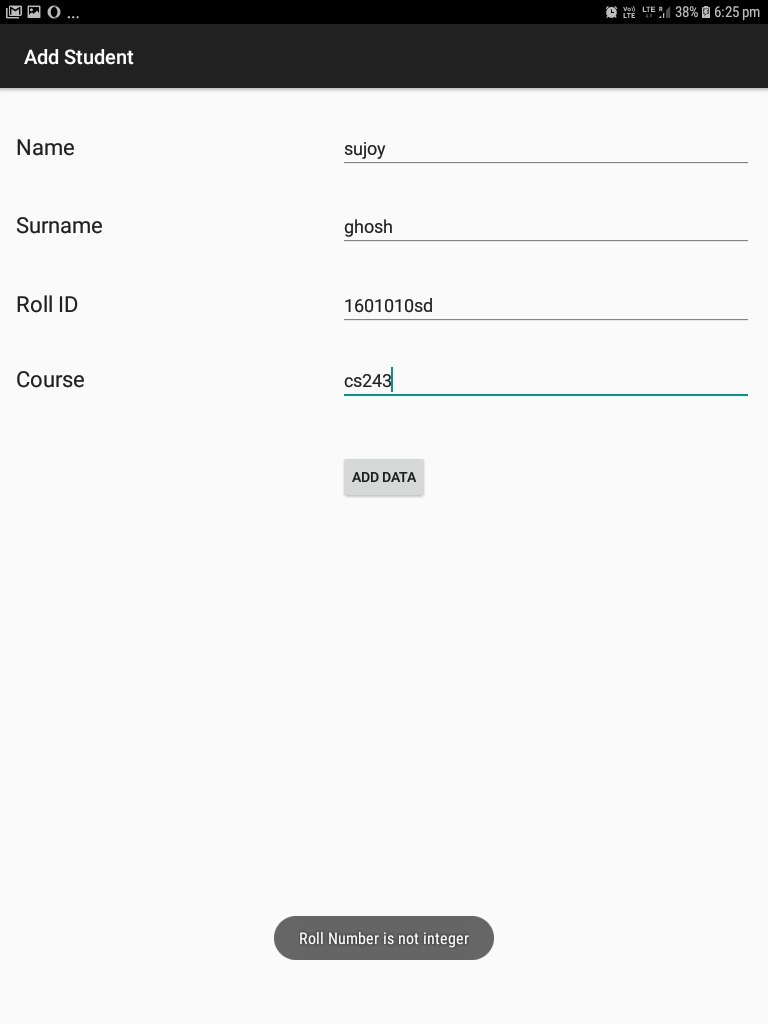
\includegraphics[width=0.42\textwidth, keepaspectratio]{addnotint.jpg}
\end{figure}
\textbf{Output}: Displays "Roll number is not integer". We get our expected output.


\item \textbf{Input}:  Roll No. already exists in entered course ID\\
\textbf{Expected Output}: Displays "Student already exists".
\begin{figure}[H]
\centering
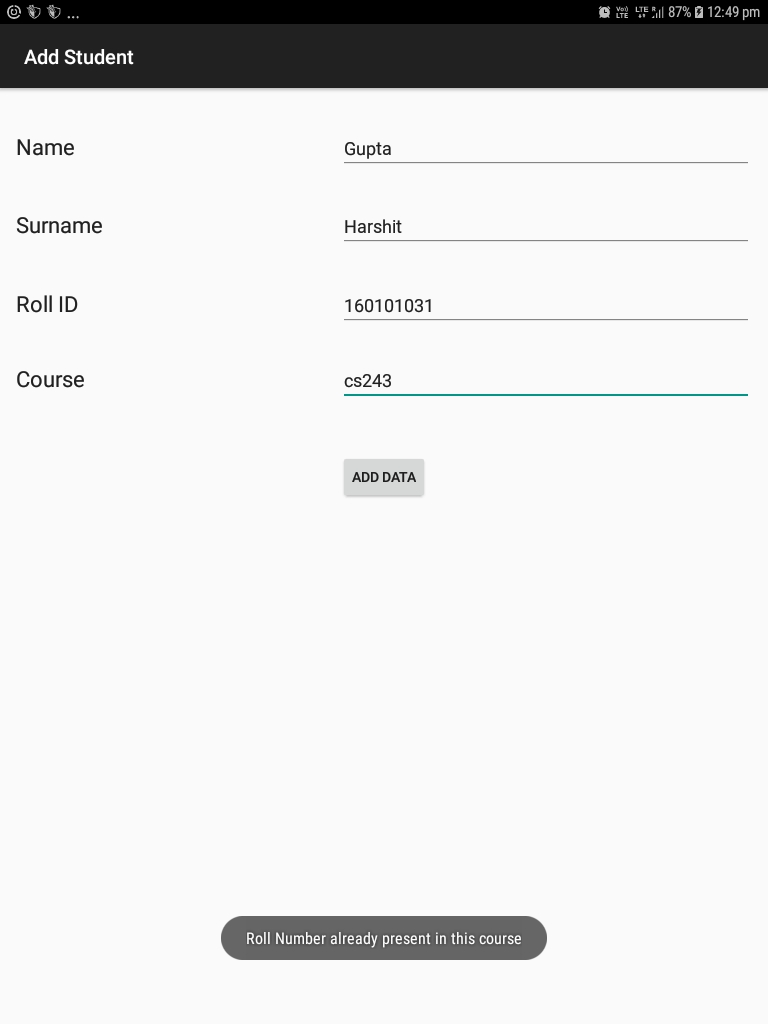
\includegraphics[width=0.42\textwidth, keepaspectratio]{addpresent.jpg}
\end{figure}
\textbf{Output}: Displays "Roll number already present in database". We get our desired output.

\item \textbf{Input}: Roll No. already exists in other course ID\\
\textbf{Expected Output}: Adds student successfully to database.
\begin{figure}[H]
\begin{subfigure}{0.5\textwidth}
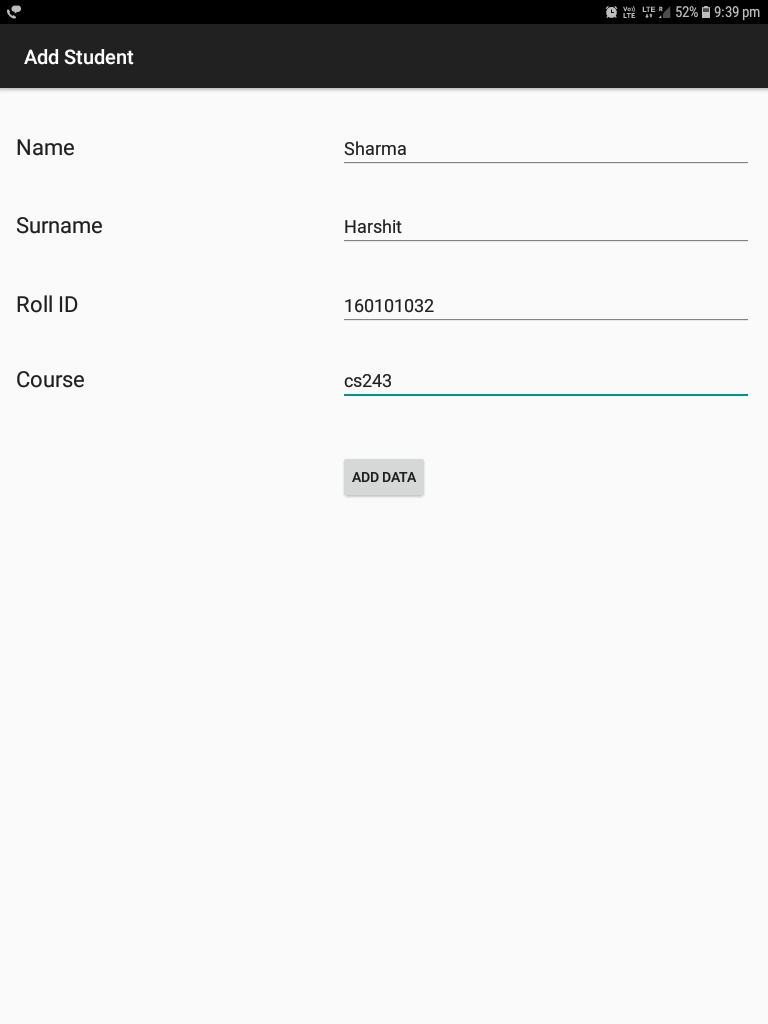
\includegraphics[width=0.85\linewidth, keepaspectratio]{addok.jpg} 
\caption{Input with correct details}
\label{fig:subim1}
\end{subfigure}
\begin{subfigure}{0.5\textwidth}
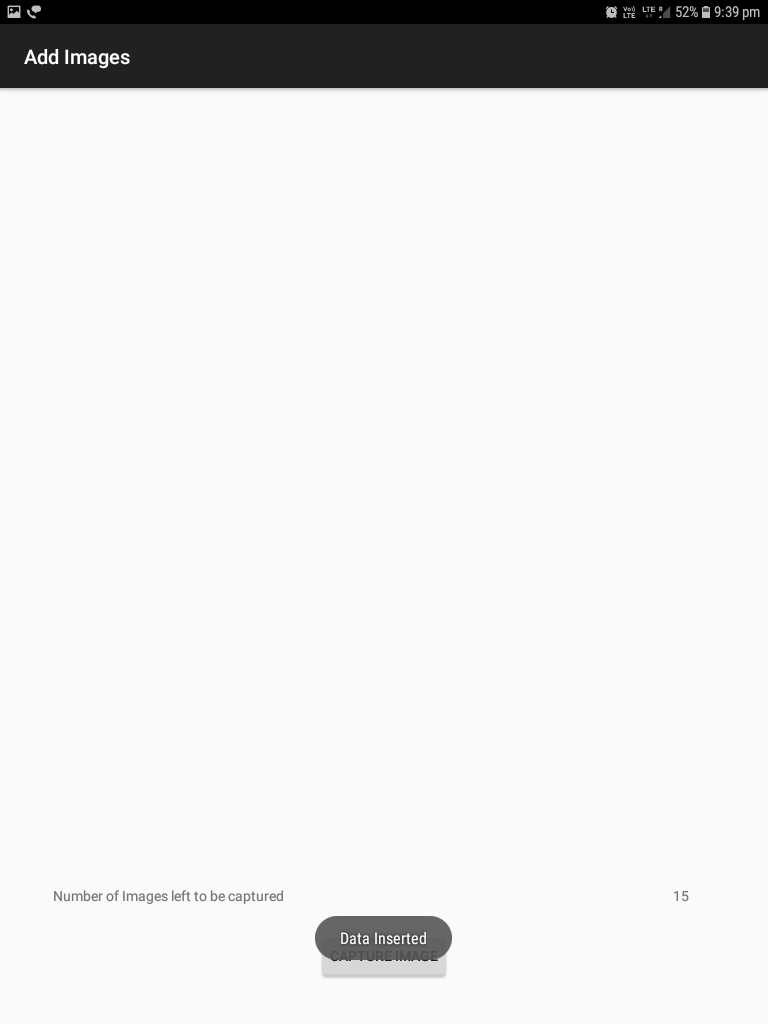
\includegraphics[width=0.85\linewidth, keepaspectratio]{added.jpg}
\caption{Output}
\label{fig:subim2}
\end{subfigure}
\end{figure}
\textbf{Output}: Displays "Data inserted". Hence, we get our desired output.
%it displays "Data inserted". Hence we get our desired output.

\item \textbf{Input}: If any one field is left empty\\
\textbf{Expected Output}: Shows error on empty fields.
\begin{figure}[H]
\begin{subfigure}{0.5\textwidth}
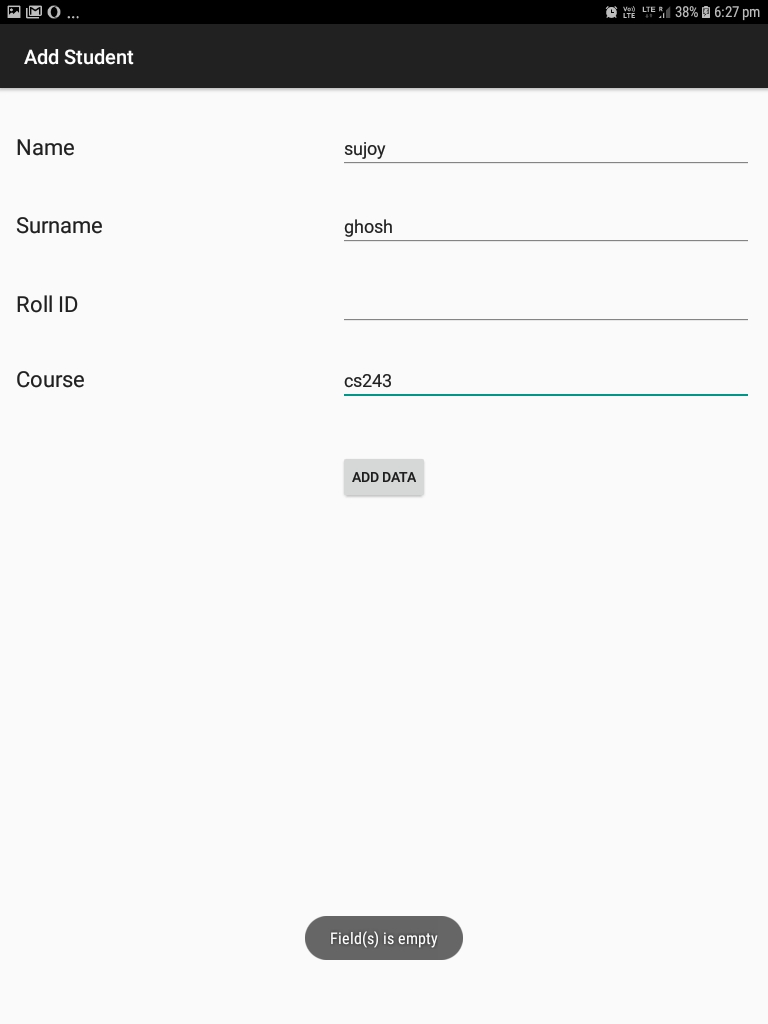
\includegraphics[width=0.85\linewidth, keepaspectratio]{addempty1.jpg} 
\label{fig:subim1}
\end{subfigure}
\begin{subfigure}{0.5\textwidth}
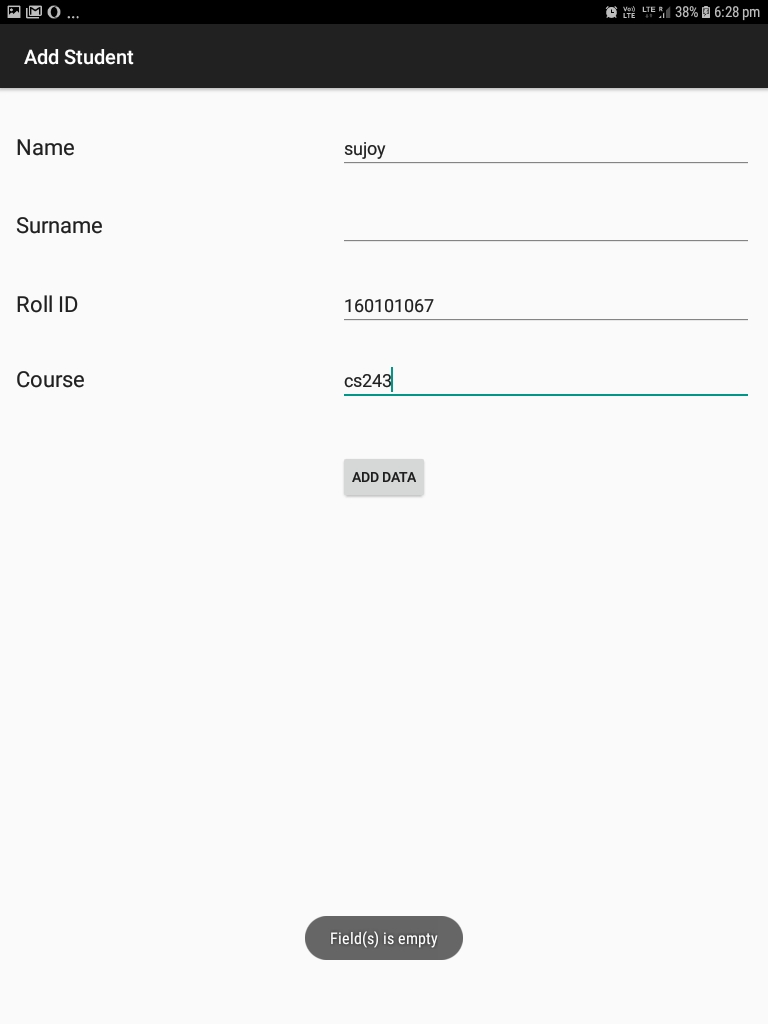
\includegraphics[width=0.85\linewidth, keepaspectratio]{addempty2.jpg}
\label{fig:subim2}
\end{subfigure}
\end{figure}
\begin{figure}[H]
\centering
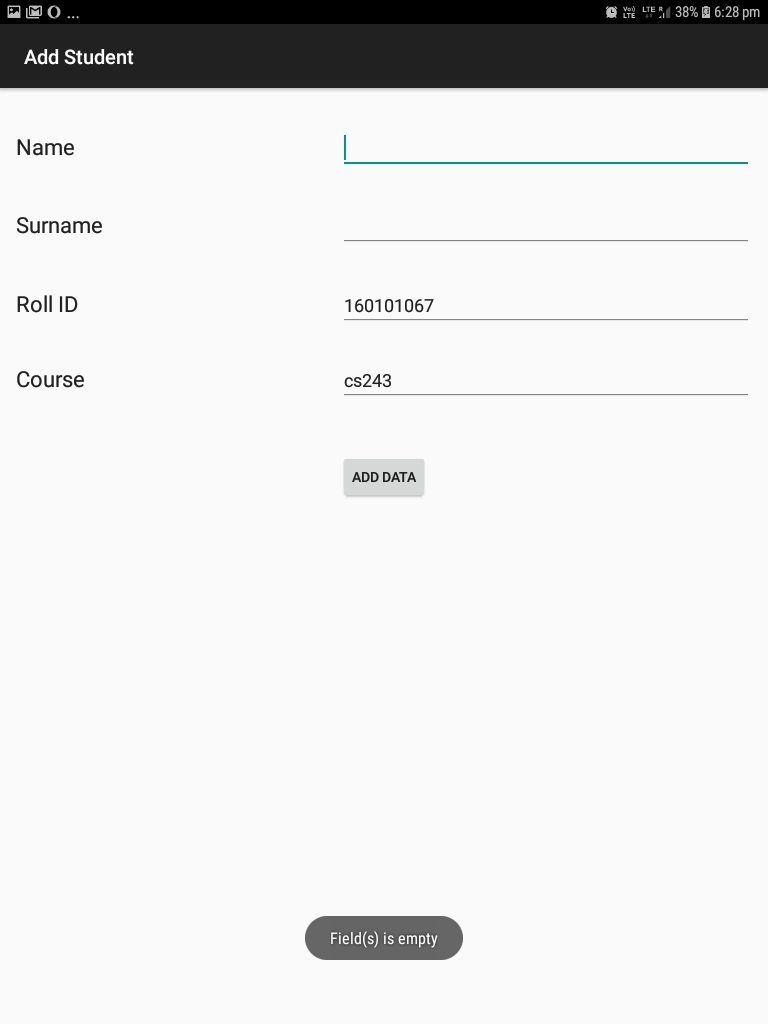
\includegraphics[width=0.42\textwidth, keepaspectratio]{addempty3.jpg}
\caption{Input with empty details}
\end{figure}
\textbf{Output}: Displays "Field(s) is empty" and doesn't insert it to database. Hence we get our desired output 
\newpage
\item \textbf{Input}: If all fields are filled correctly and input does not belong to any of the above class.\\
\textbf{Expected Output}: Displays "Student Record created successfully".
\begin{figure}[H]
\begin{subfigure}{0.5\textwidth}
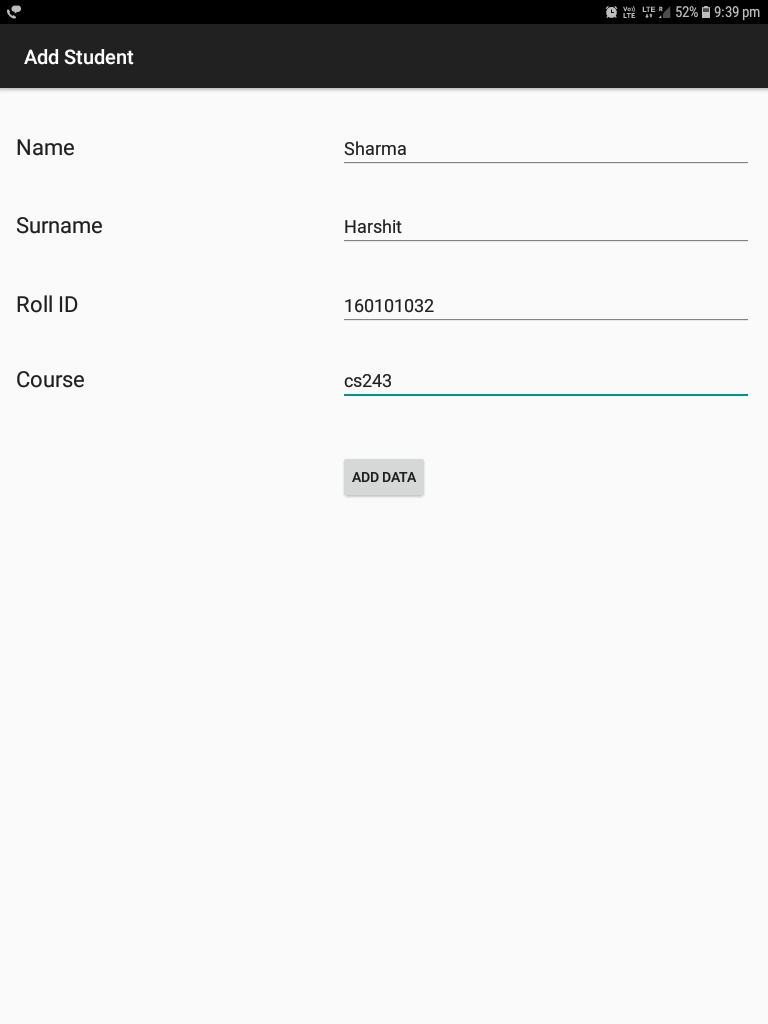
\includegraphics[width=0.85\linewidth, keepaspectratio]{addok.jpg} 
\caption{Input with correct details}
\label{fig:subim1}
\end{subfigure}
\begin{subfigure}{0.5\textwidth}
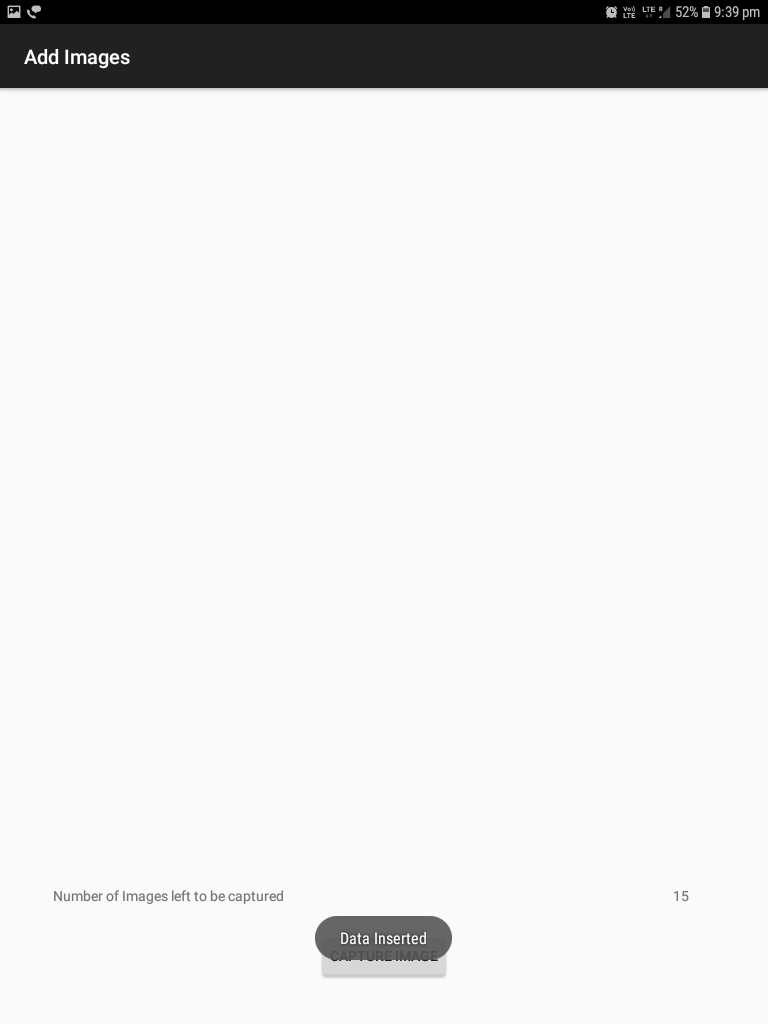
\includegraphics[width=0.85\linewidth, keepaspectratio]{added.jpg}
\caption{Output}
\label{fig:subim2}
\end{subfigure}
\caption{We get desired output}
\end{figure}
\textbf{Output}: It displays "Data inserted". Hence we get our desired output.

\end{enumerate}
%\item[•]\textbf{Boundary Cases}: Equivalence classes here are discrete. There are no boundary cases.
\end{itemize}

\section{Module Name: Add Images}
\begin{itemize}
\item[•]\textbf{Equivalence Classes}:
\begin{enumerate}
\item \textbf{Input}: No. of added images $<$ 15 \\
\textbf{Expected Output}: Option to return to main menu is not shown.
\begin{figure}[H]
\centering
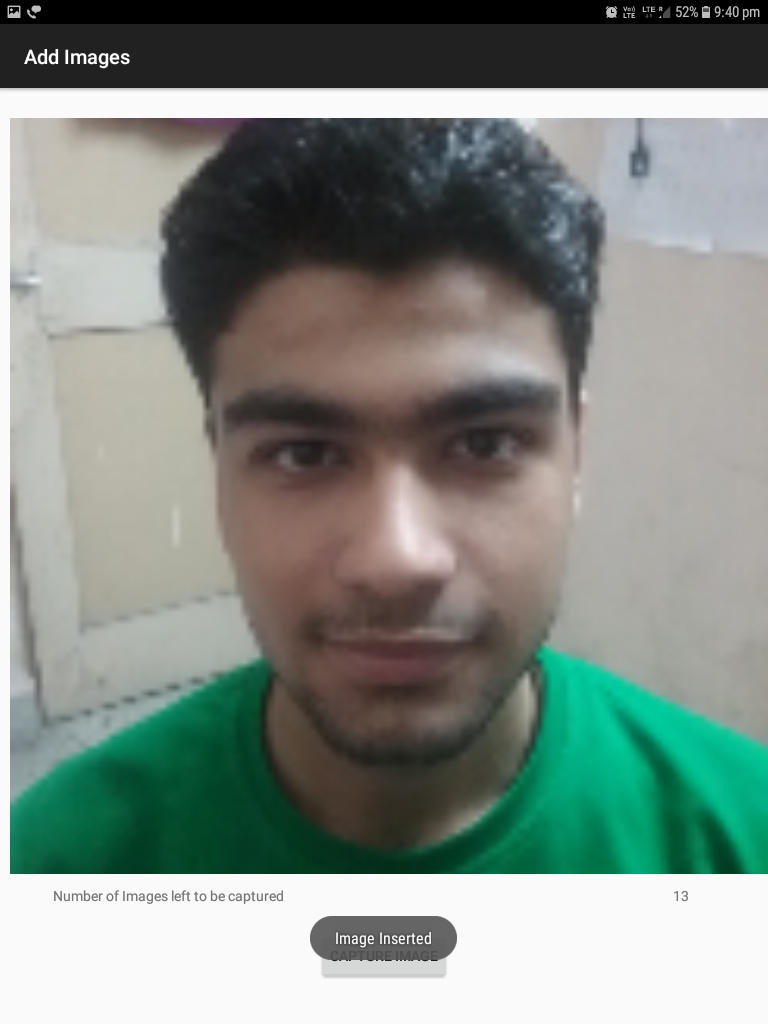
\includegraphics[width=0.42\textwidth, keepaspectratio]{imgadd.jpg}
\end{figure}
\textbf{Output}: Option to return to main menu is not shown. Hence we get our desired output.

\item \textbf{Input}:  No. of added images $>$ 15\\
\textbf{Expected Output}: Clicking more than 15 images should not be allowed.
\begin{figure}[H]
\centering
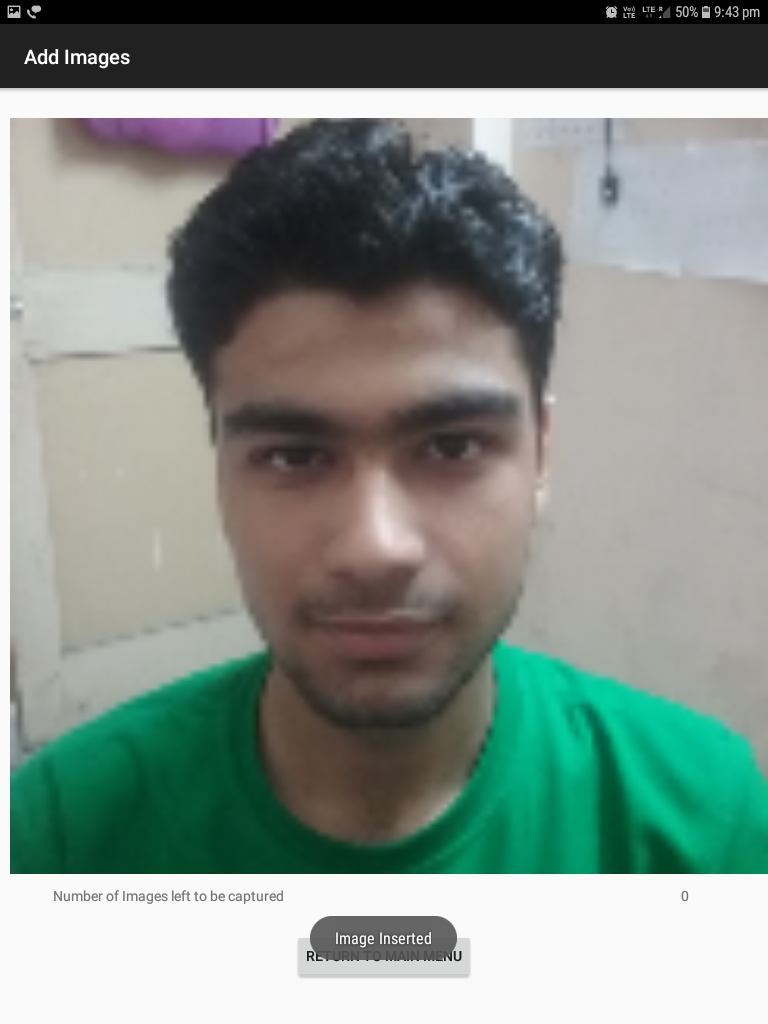
\includegraphics[width=0.42\textwidth, keepaspectratio]{imgboun.jpg}
\end{figure}
\textbf{Output}: Return to main menu is shown when images$=$15. Hence we get our desired output.

\end{enumerate}
\item[•]\textbf{Boundary Cases}:
\begin{enumerate}
\item \textbf{Input}: No. of added images $=$ 15 \\
\textbf{Expected Output}: Gives option to return to main screen.
\begin{figure}[H]
\centering
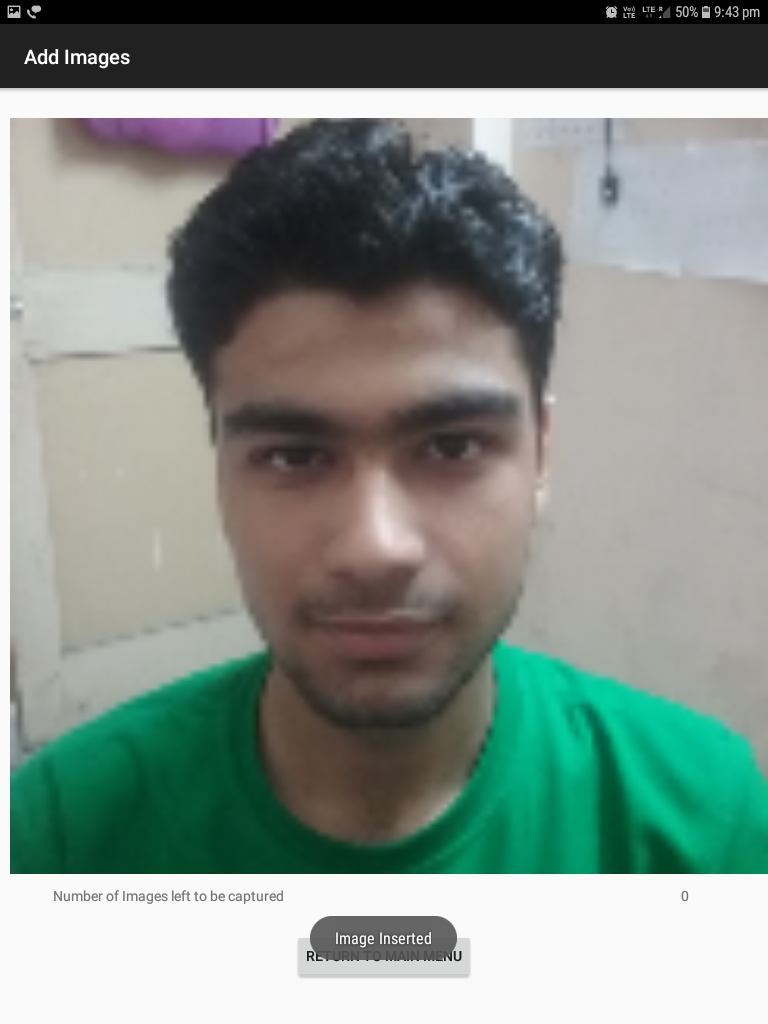
\includegraphics[width=0.42\textwidth, keepaspectratio]{imgboun.jpg}
\caption{Number of photos left $=$ 0}
\end{figure}
\textbf{Output}: Return to main menu is shown when images$=$15. Hence we get our desired output.

\end{enumerate}
\end{itemize}

\section{Module Name: Edit Student}
\begin{itemize}
\item[•]\textbf{Equivalence Classes}:
\begin{enumerate}
\item \textbf{Input}: Roll No. not integer \\
\textbf{Expected Output}: Displays "Roll Number is not an integer".
\begin{figure}[H]
\centering
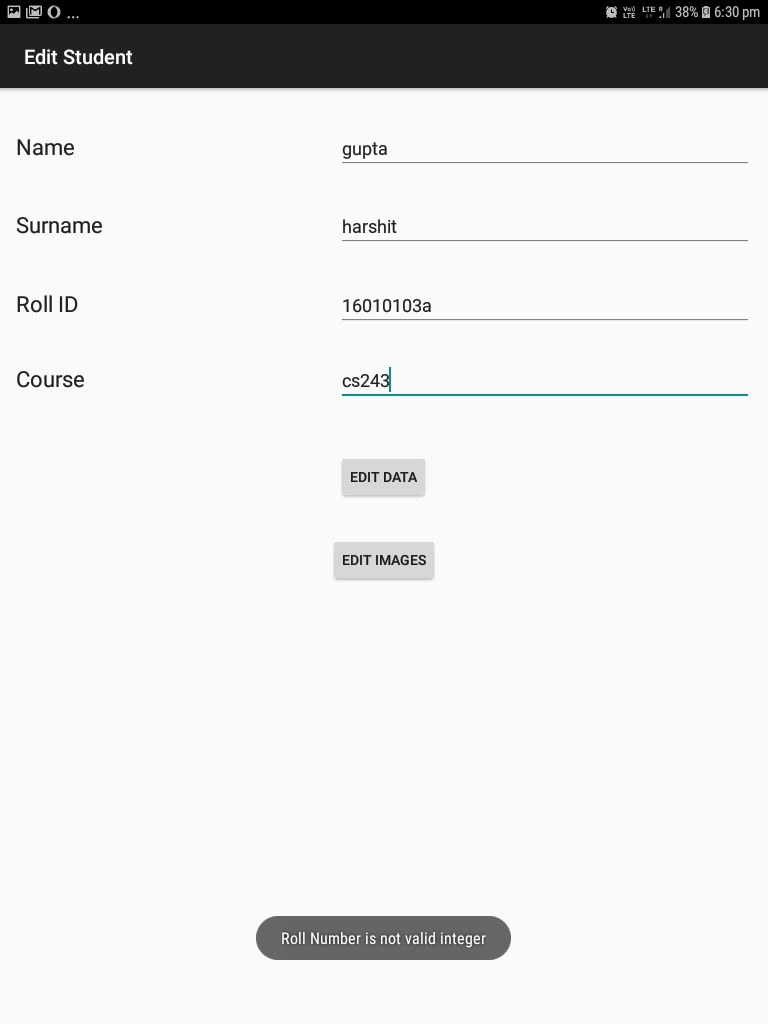
\includegraphics[width=0.42\textwidth, keepaspectratio]{editrollnot.jpg}
\end{figure}
\textbf{Output}: Displays "Roll Number is not an integer".We get our desired output.

\item \textbf{Input}:  Roll No. already exists but in other course ID\\
\textbf{Expected Output}: Displays "Student does not exists".
\begin{figure}[H]
\begin{subfigure}{0.5\textwidth}
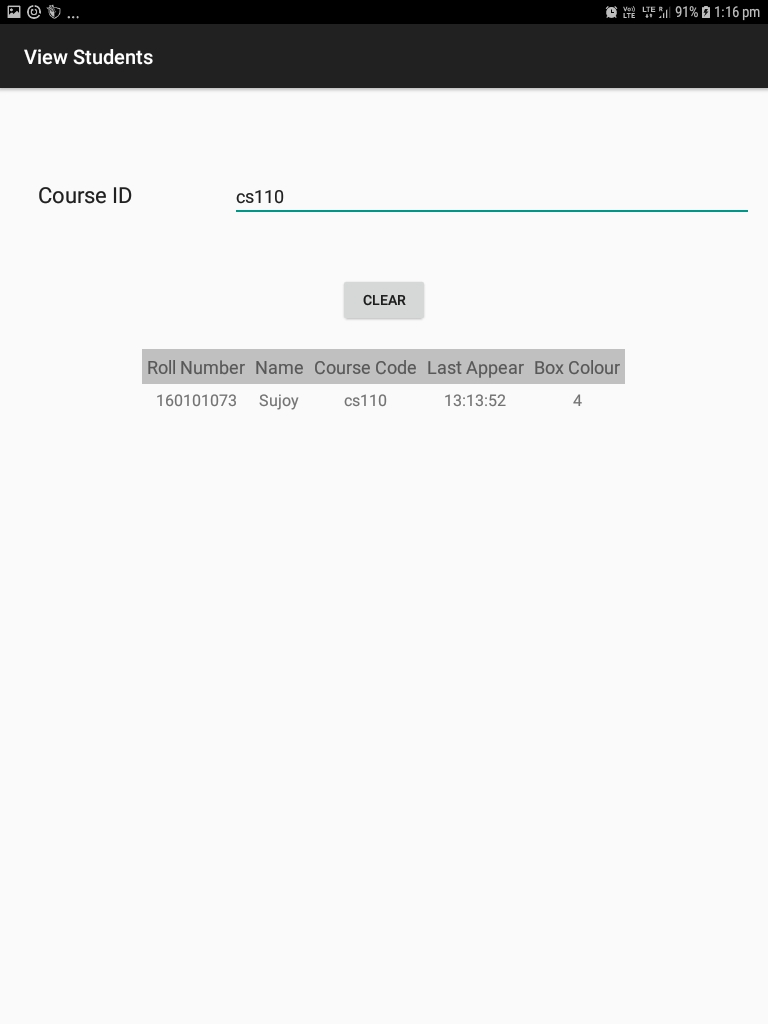
\includegraphics[width=0.85\linewidth, keepaspectratio]{deleteshow.jpg} 
\caption{Input with correct details}
\label{fig:subim1}
\end{subfigure}
\begin{subfigure}{0.5\textwidth}
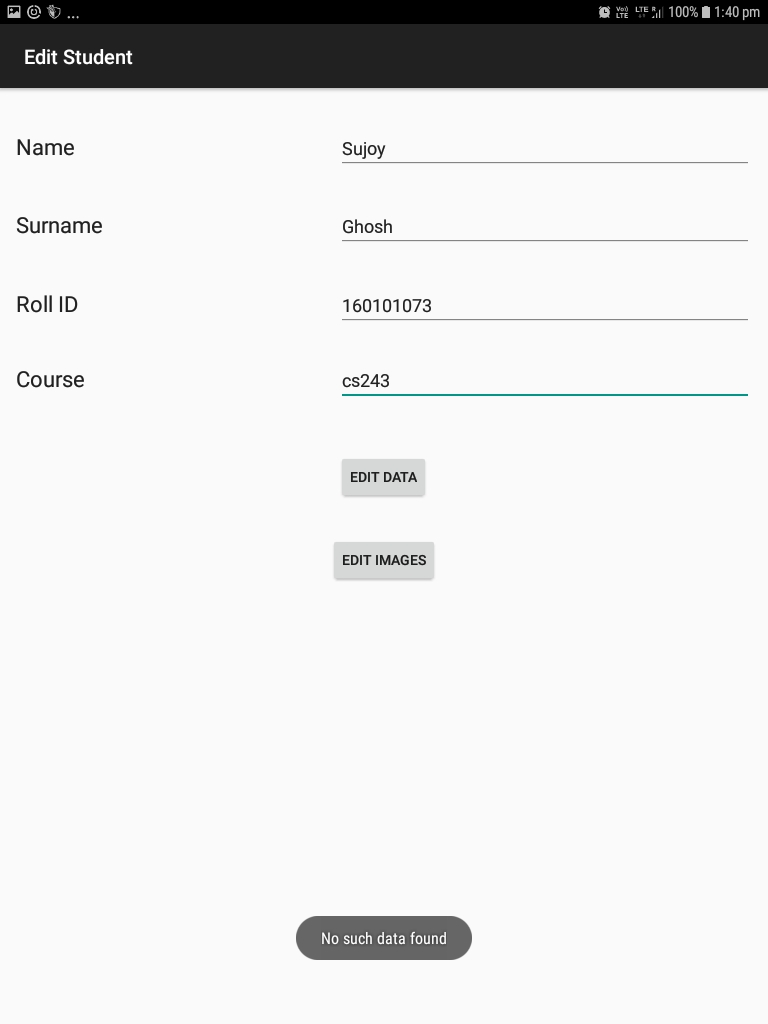
\includegraphics[width=0.85\linewidth, keepaspectratio]{editnana.jpg}
\caption{Output}
\label{fig:subim2}
\end{subfigure}
\end{figure}
\textbf{Output}: Displays "No such data found".We get our desired output.


\item \textbf{Input}:  Roll No. doesn't exist\\
\textbf{Expected Output}:  Displays "Student does not exists".
\begin{figure}[H]
\centering
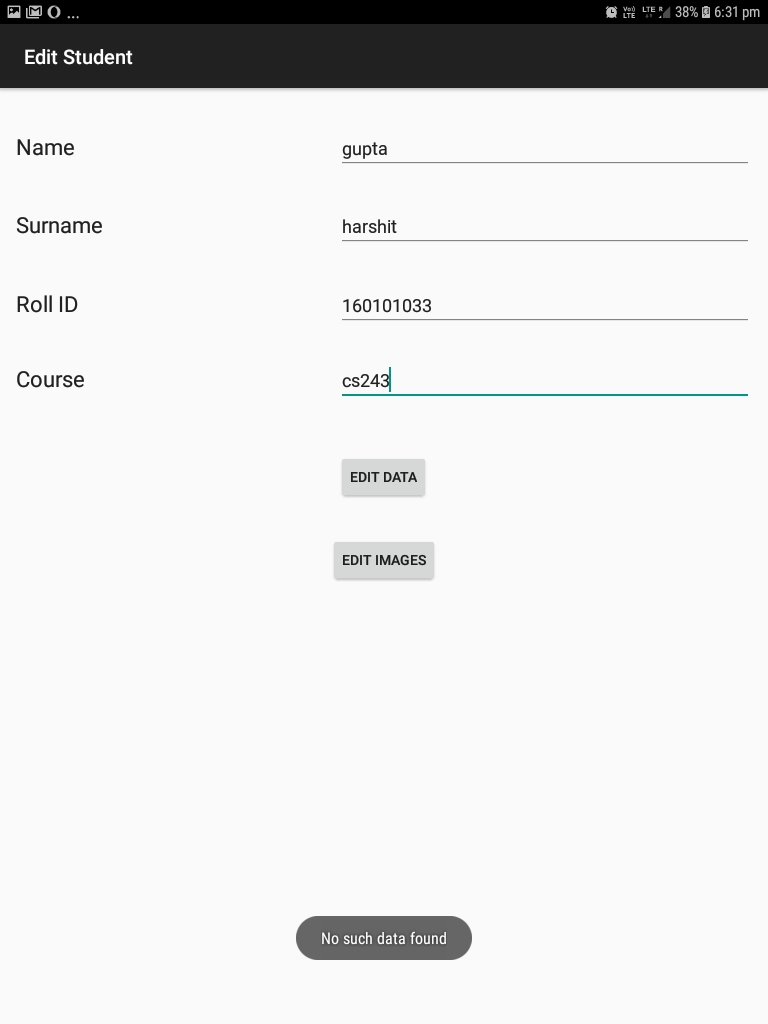
\includegraphics[width=0.4\textwidth, keepaspectratio]{editnoexist.jpg}
\end{figure}
\textbf{Output}: Displays "No such data found". Hence, we get our desired output.

\item \textbf{Input}: If any one field is left empty\\
\textbf{Expected Output}: Shows error on empty fields.
\begin{figure}[H]
\begin{subfigure}{0.5\textwidth}
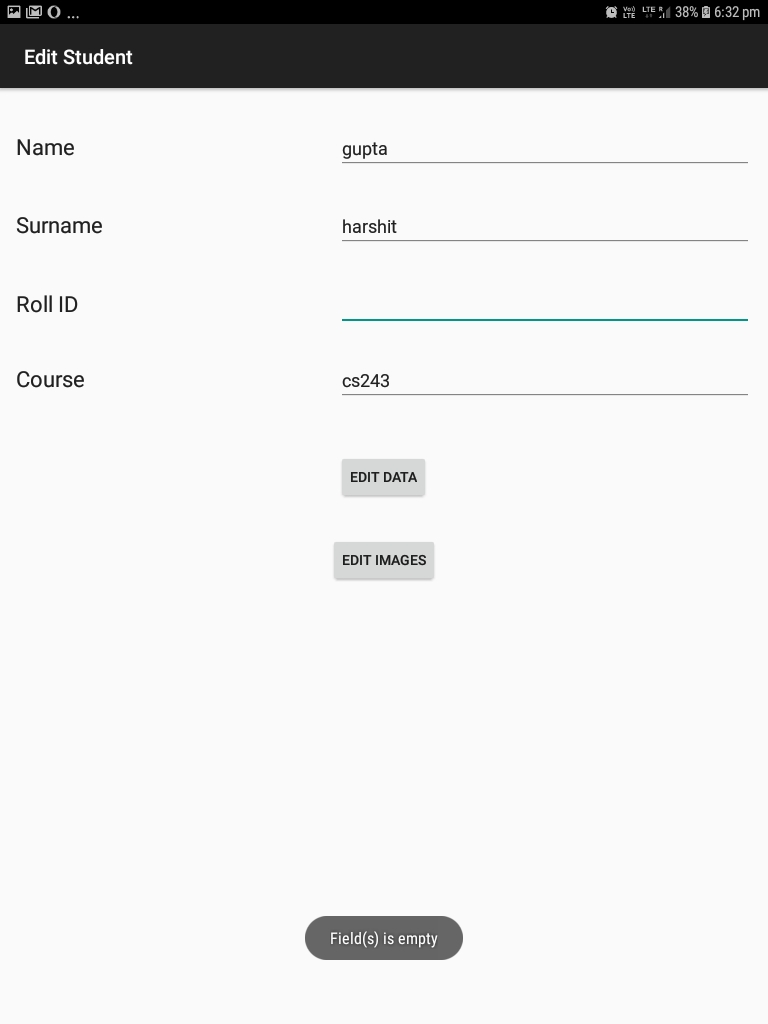
\includegraphics[width=0.85\linewidth, keepaspectratio]{editempty1.jpg} 
\caption{Input with empty fields}
\label{fig:subim1}
\end{subfigure}
\begin{subfigure}{0.5\textwidth}
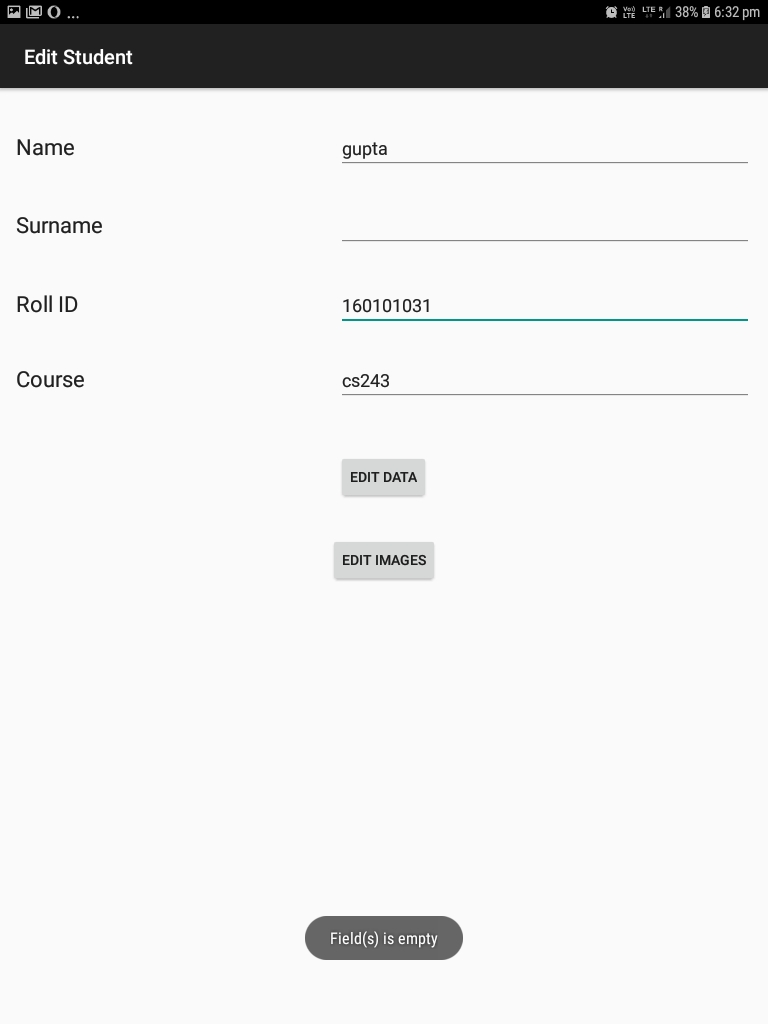
\includegraphics[width=0.85\linewidth, keepaspectratio]{editempty2.jpg}
\caption{Output}
\label{fig:subim2}
\end{subfigure}
\end{figure}
\begin{figure}[H]
\centering
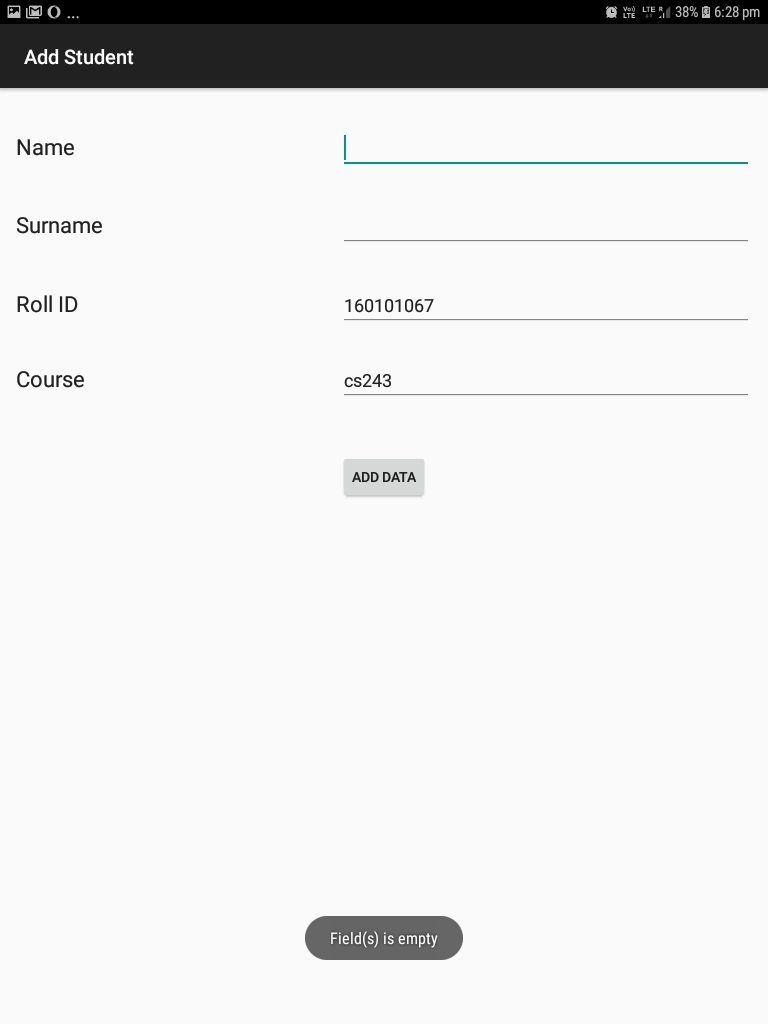
\includegraphics[width=0.42\textwidth, keepaspectratio]{addempty3.jpg}
\end{figure}
\textbf{Output}: Displays "Field(s) is empty".We get our desired output.

\item \textbf{Input}: If all fields are filled correctly and it does not belong to any of the above class.\\
\textbf{Expected Output}: Displays "Data successfully updated".
\begin{figure}[H]
\begin{subfigure}{0.5\textwidth}
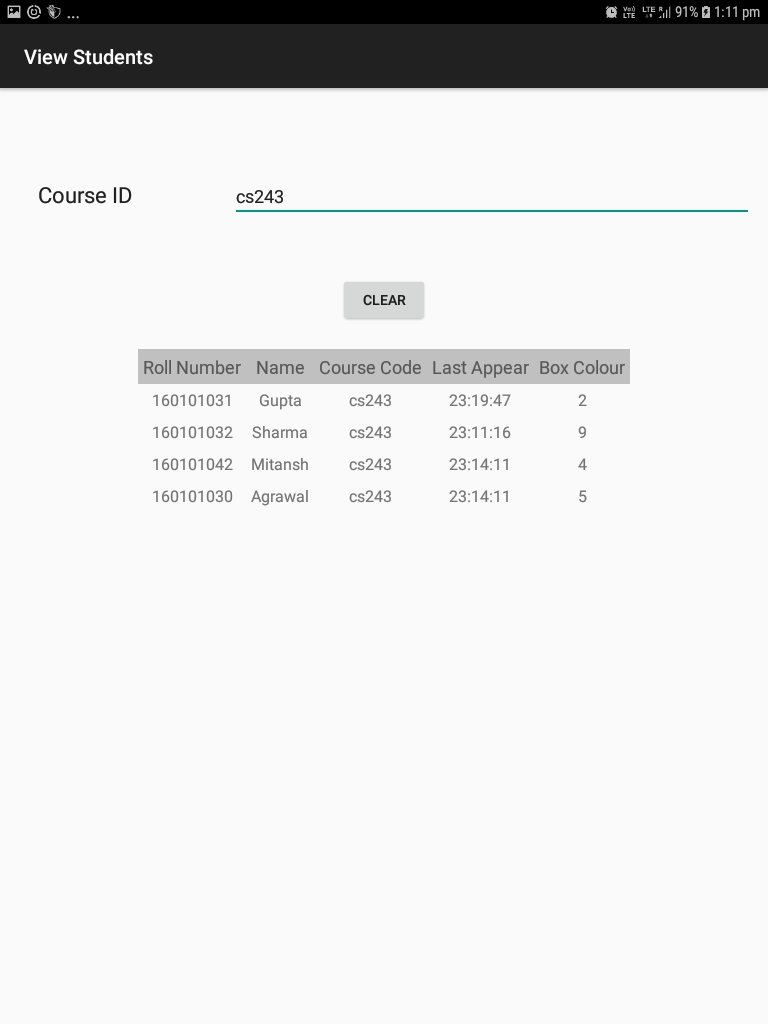
\includegraphics[width=0.85\linewidth, keepaspectratio]{viewdone.jpg} 
\caption{Student list}
\label{fig:subim1}
\end{subfigure}
\begin{subfigure}{0.5\textwidth}
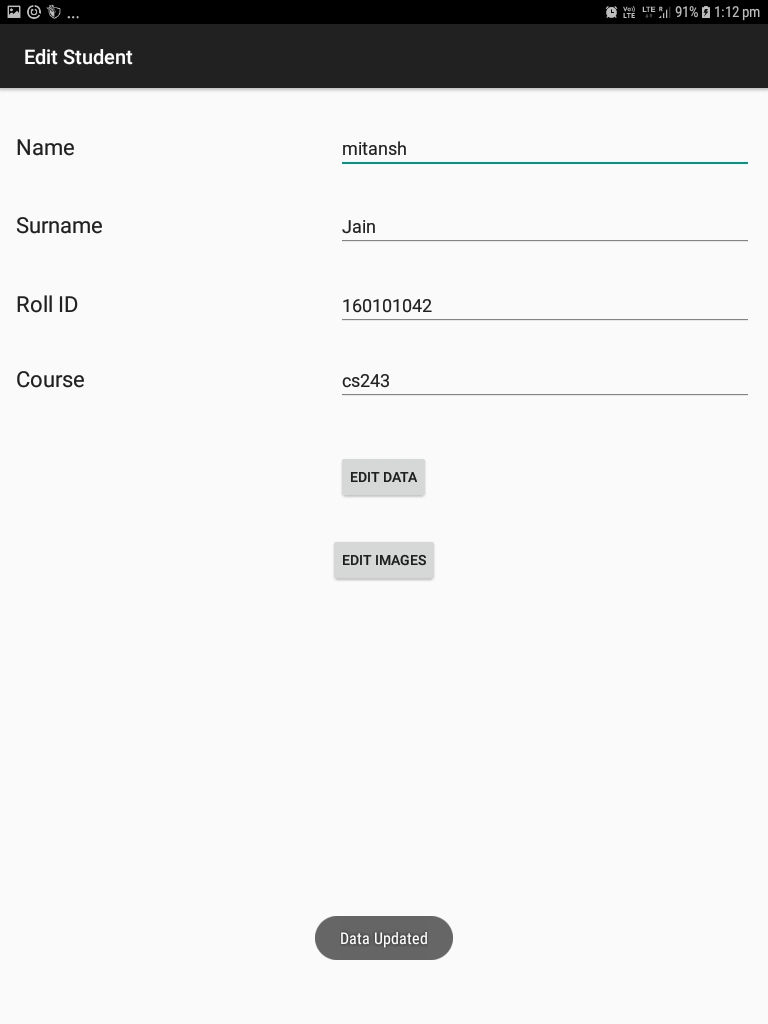
\includegraphics[width=0.85\linewidth, keepaspectratio]{editdone.jpg}
\caption{Output}
\label{fig:subim2}
\end{subfigure}
\end{figure}
\begin{figure}[H]
\centering
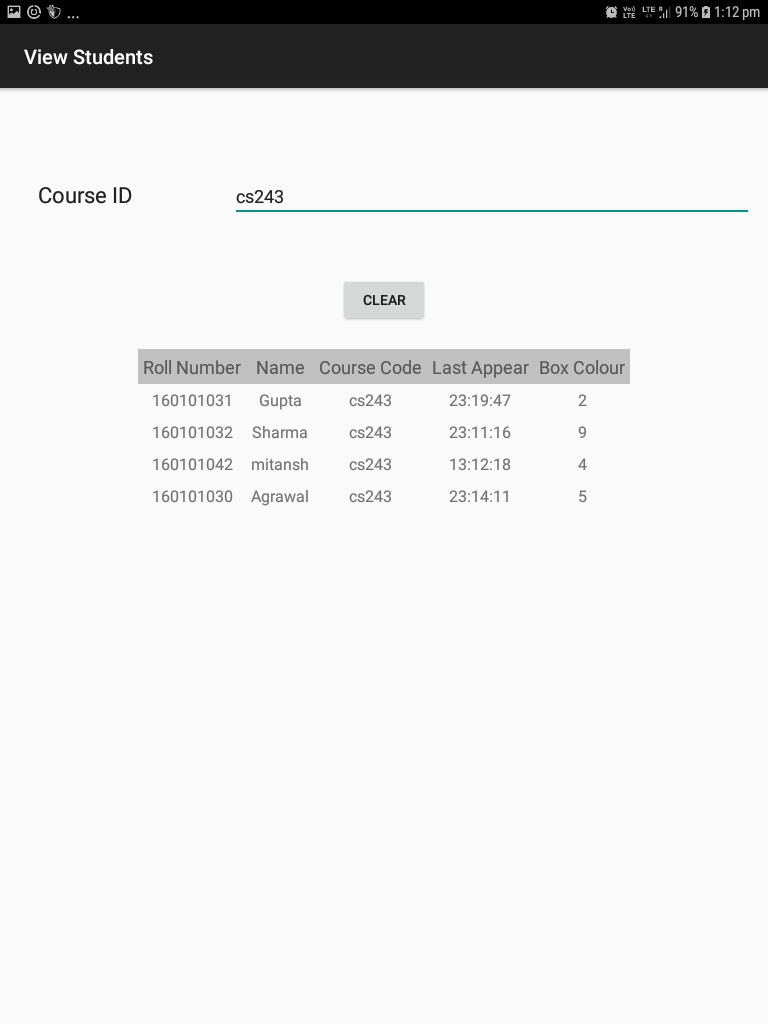
\includegraphics[width=0.42\textwidth, keepaspectratio]{editafter.jpg}
\caption{Updated List}
\end{figure}
\textbf{Output}: Displays "Data Updated".Student list was also updated.We get our desired output.

\end{enumerate}
%\item[•]\textbf{Boundary Cases}: Equivalence classes here are discrete. There are no boundary cases.
\end{itemize}

\section{Module Name: View Student List}
\begin{itemize}
\item[•]\textbf{Equivalence Classes}:
\begin{enumerate}
\item \textbf{Input}: Course ID field is left empty\\
\textbf{Expected Output}: Shows error on empty field.
\begin{figure}[H]
\centering
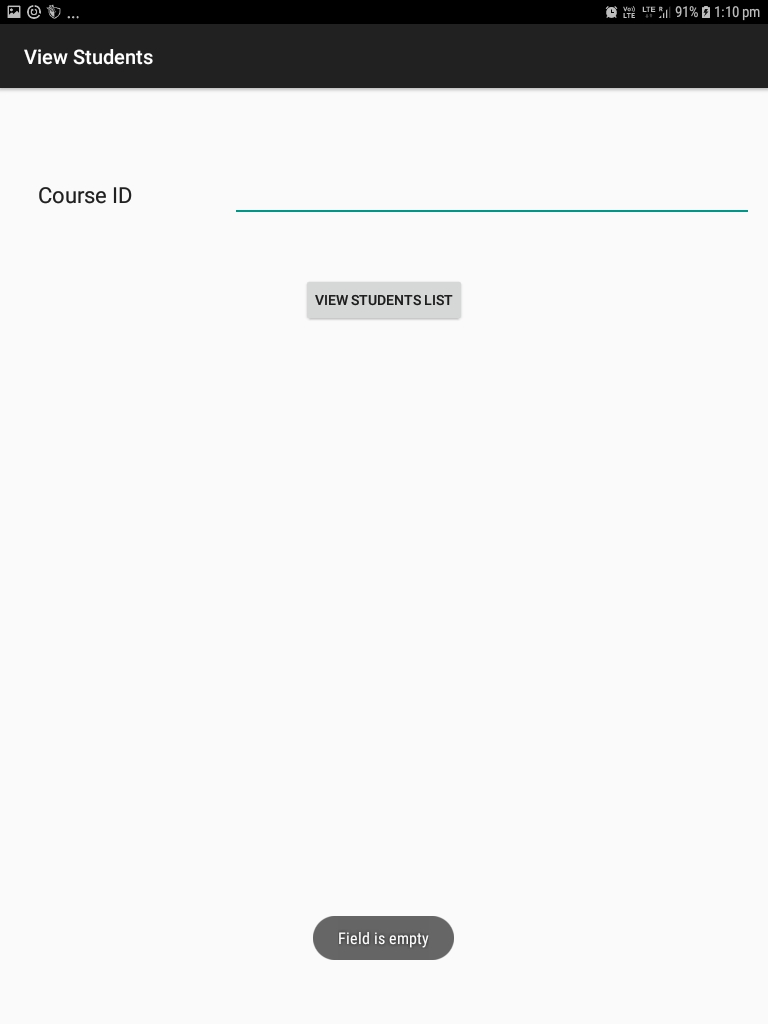
\includegraphics[width=0.42\textwidth, keepaspectratio]{viewempty.jpg}
\end{figure}
\textbf{Output}: Displays "Field is empty".We get our desired output.

\item \textbf{Input}: Invalid Course ID\\
\textbf{Expected Output}: Displays "no such course Id exists".
\begin{figure}[H]
\centering
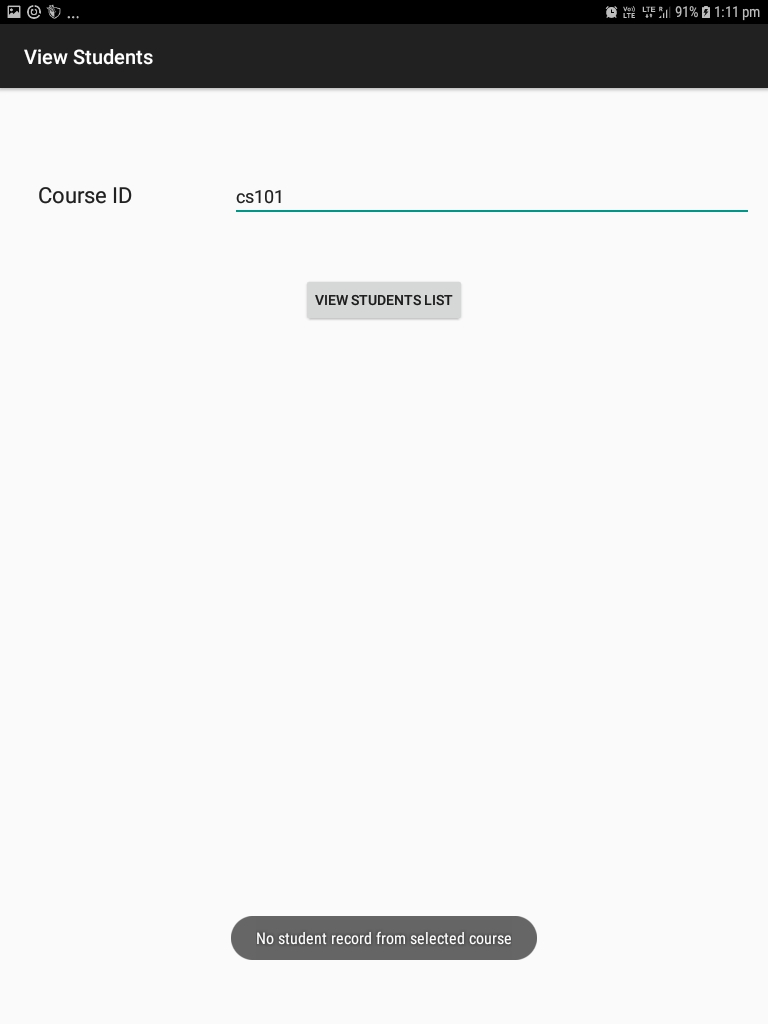
\includegraphics[width=0.42\textwidth, keepaspectratio]{viewnot.jpg}
\caption{Input with incorrect course id}
\end{figure}
\textbf{Output}: Displays "No student record from selected course".We get our desired output.

\item \textbf{Input}:  Valid Course ID\\
\textbf{Expected Output}: Displays list of all student that were added to data base.
\begin{figure}[H]
\centering
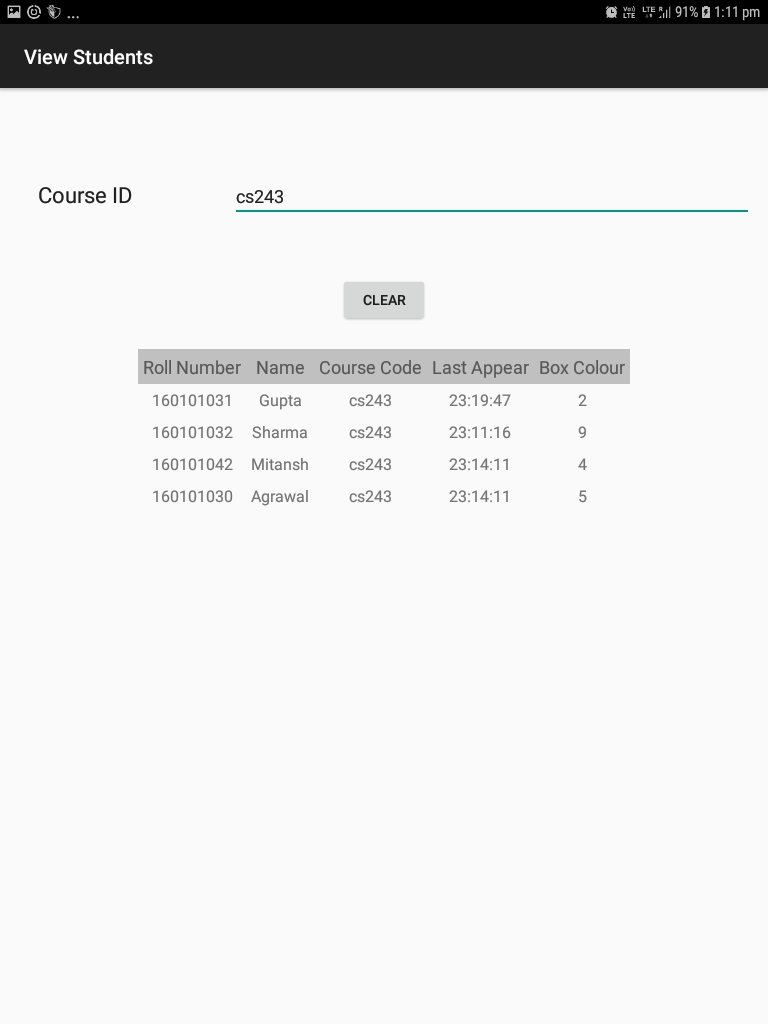
\includegraphics[width=0.42\textwidth, keepaspectratio]{viewdone.jpg}
\caption{Input with corrected course id}
\end{figure}
\textbf{Output}: Displays the list of students.We get our desired output.

\end{enumerate}
%\item[•]\textbf{Boundary Cases}: Equivalence classes here are discrete. There are no boundary cases.
\end{itemize}

\section{Module Name: Delete Student Record}
\begin{itemize}
\item[•]\textbf{Equivalence Classes}:
\begin{enumerate}
\item \textbf{Input}: Roll No. not an integer\\
\textbf{Expected Output}: Displays "Roll Number not an integer".
\begin{figure}[H]
\centering
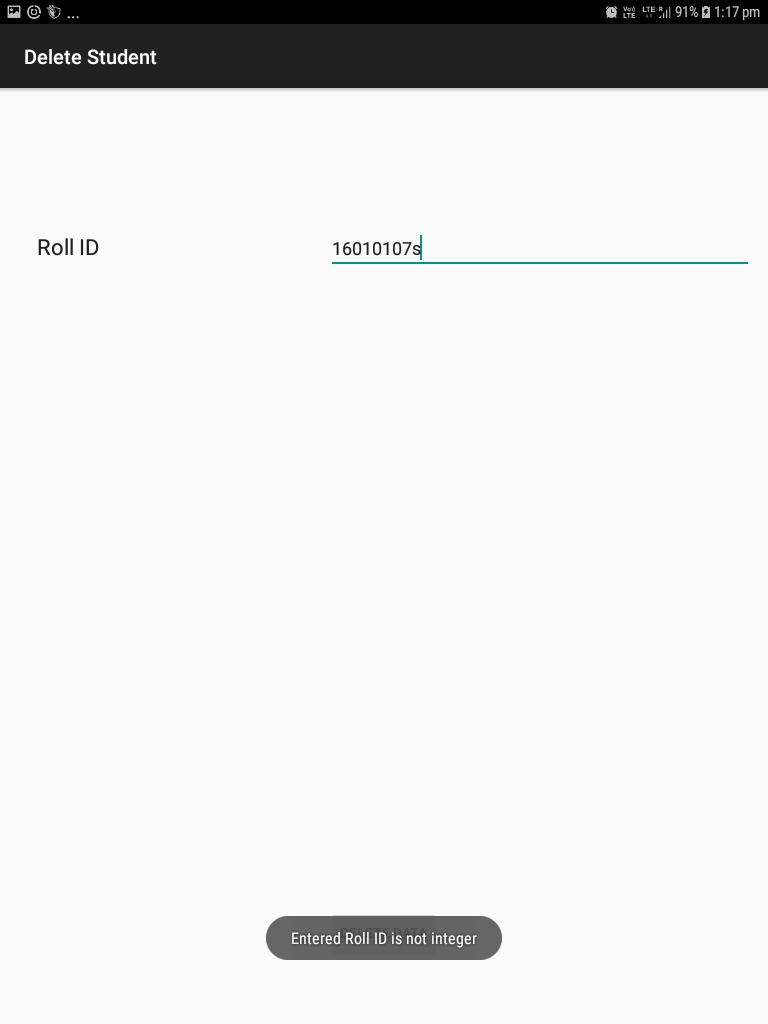
\includegraphics[width=0.42\textwidth, keepaspectratio]{deleteinvalid.jpg}
\end{figure}
\textbf{Output}: Displays "Roll Number is not an integer".We get our desired output.

\item \textbf{Input}: Roll No.doesn't exists.\\
\textbf{Expected Output}: Displays "Roll Number does not exist". 
\begin{figure}[H]
\centering
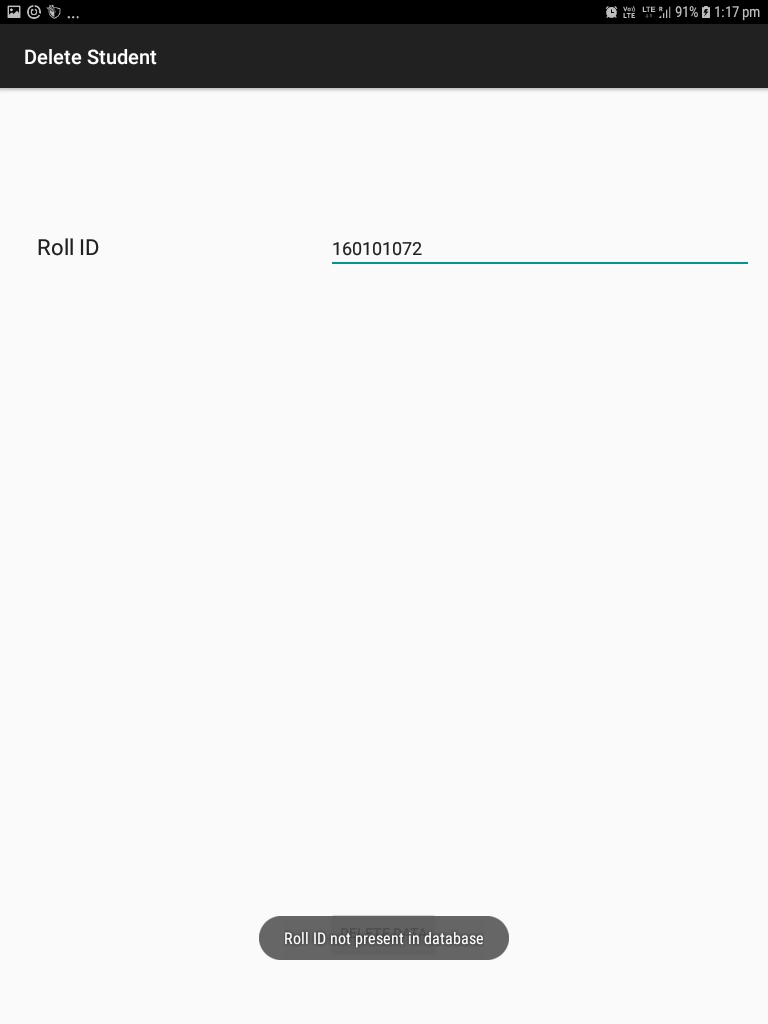
\includegraphics[width=0.42\textwidth, keepaspectratio]{deletenot.jpg}
\end{figure}
\textbf{Output}: Displays "Roll Number not in database". We get our desired output.

\item \textbf{Input}: Roll No. exists.\\
\textbf{Expected Output}: Displays "Data deleted". Roll Number should not be visible in table of students in from view student list module. 
\begin{figure}[H]
\begin{subfigure}{0.5\textwidth}
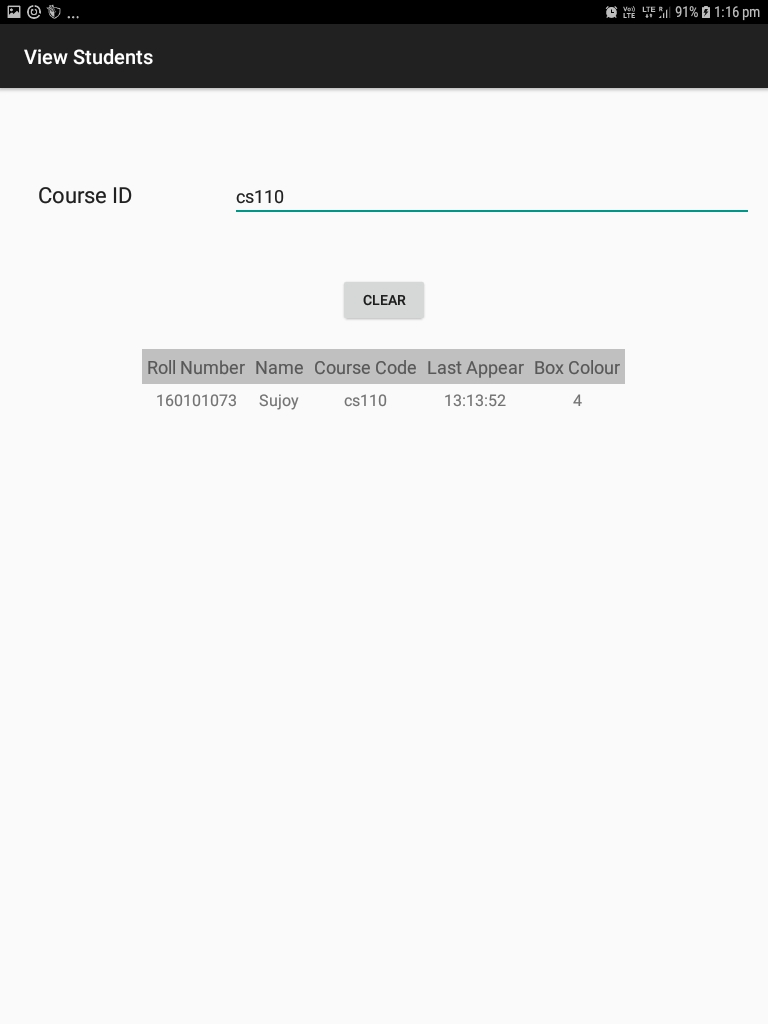
\includegraphics[width=0.85\linewidth, keepaspectratio]{deleteshow.jpg} 
\caption{Student List}
\label{fig:subim1}
\end{subfigure}
\begin{subfigure}{0.5\textwidth}
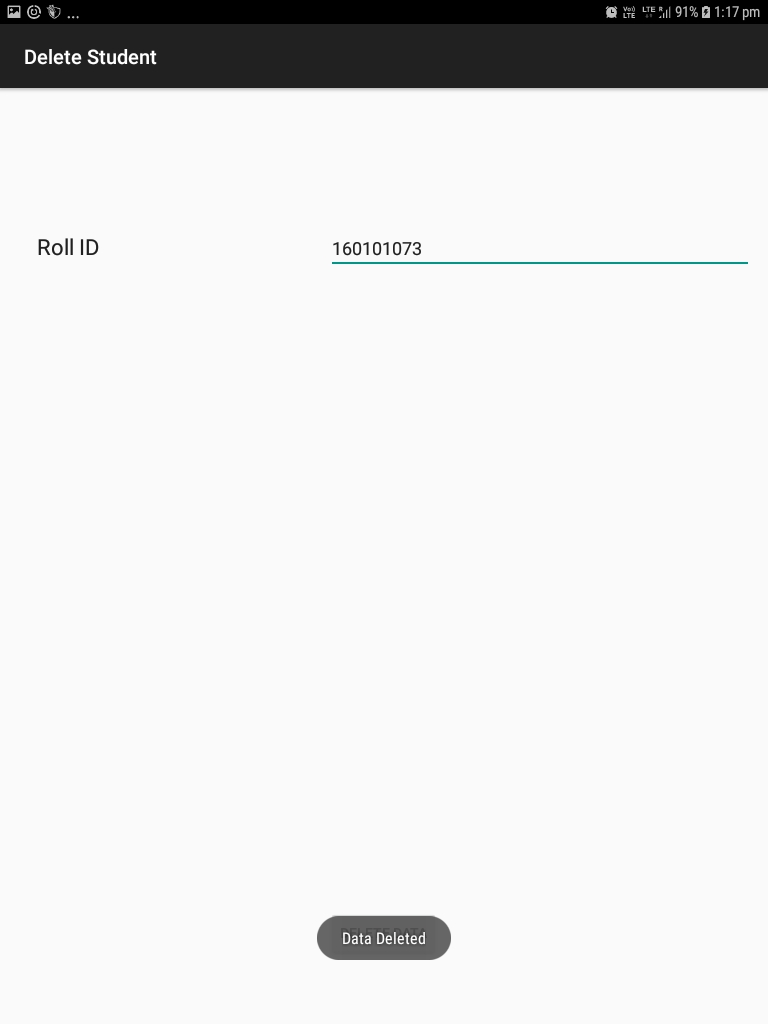
\includegraphics[width=0.85\linewidth, keepaspectratio]{deletedone.jpg}
\caption{Output}
\label{fig:subim2}
\end{subfigure}
\end{figure}
\textbf{Output}: Displays "Data Deleted".We get our desired output.
\end{enumerate}
%\item[•]\textbf{Boundary Cases}: Equivalence classes here are discrete. There are no boundary cases.
\end{itemize}

\section{Module name: Camera Session and Face Recognition}
\begin{itemize}
\item[•]\textbf{Equivalence Classes}:
\begin{enumerate}
\item \textbf{Input}: State of student $<$ 5.\\
\textbf{Expected Output}: Bounding box color: red
\begin{figure}[H]
\centering
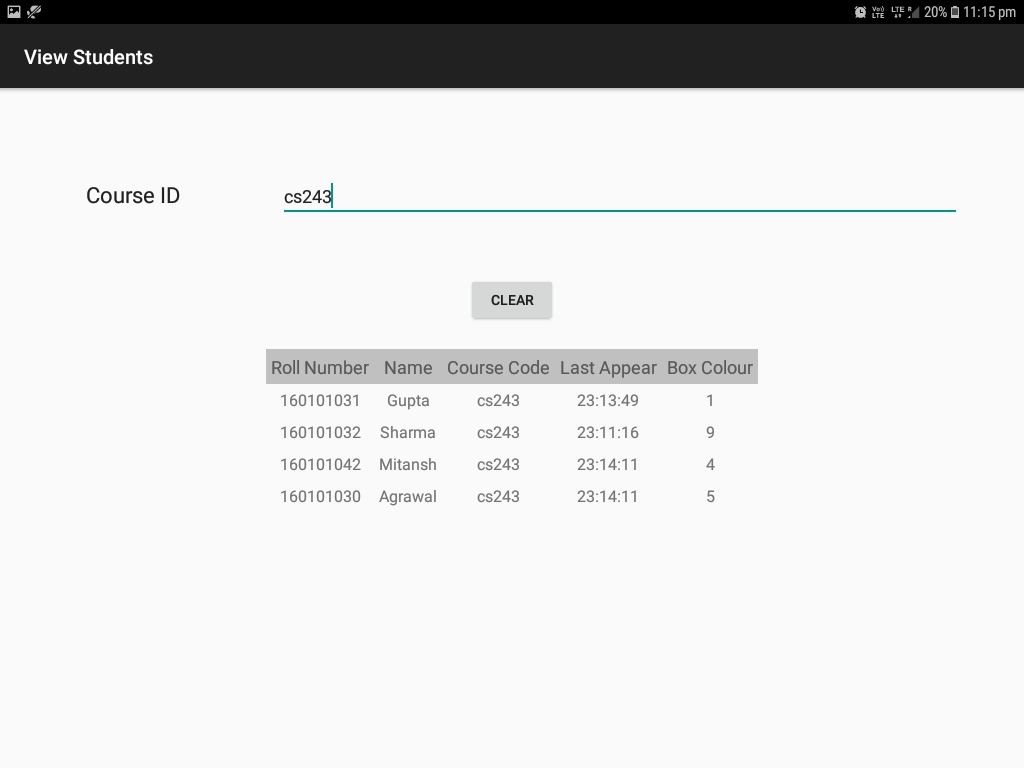
\includegraphics[width=0.7\textwidth, keepaspectratio]{camstate.jpg}
\end{figure}
\begin{figure}[H]
\centering
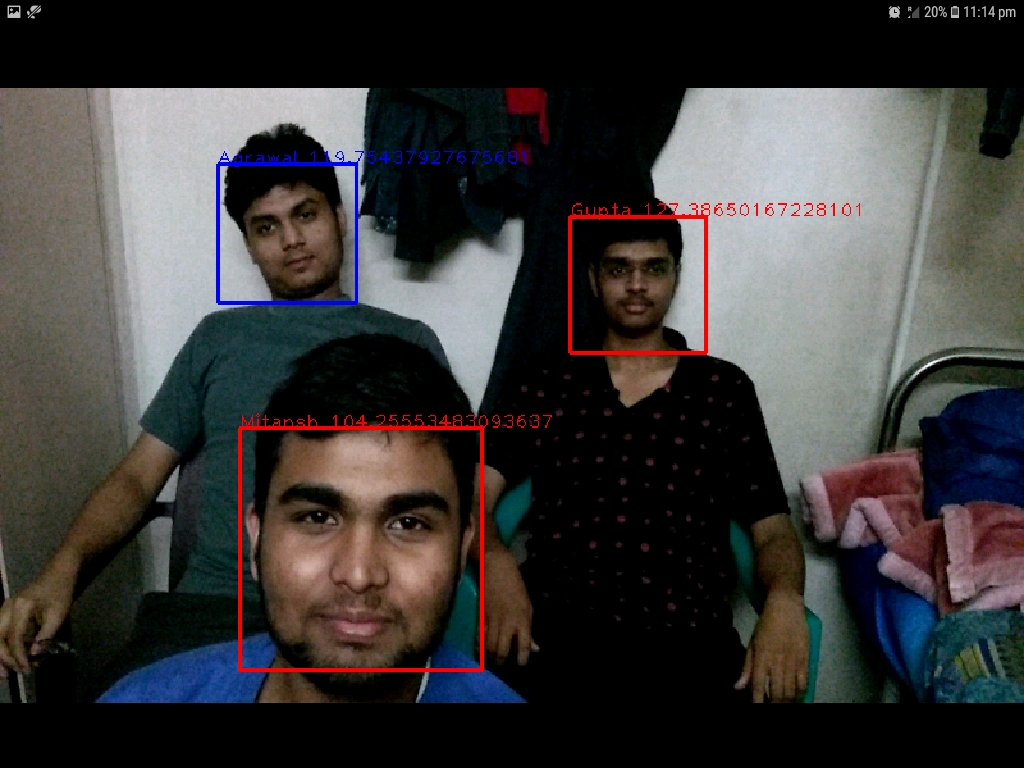
\includegraphics[width=0.7\textwidth, keepaspectratio]{cam3stud.jpg}
\end{figure}
\textbf{Output}: Displays person recognised with corresponding bounding box.We get our desired output.

\item \textbf{Input}: 5 $<$ State of student $<$ 8\\
\textbf{Expected Output}: Bounding box color: blue
\begin{figure}[H]
\centering
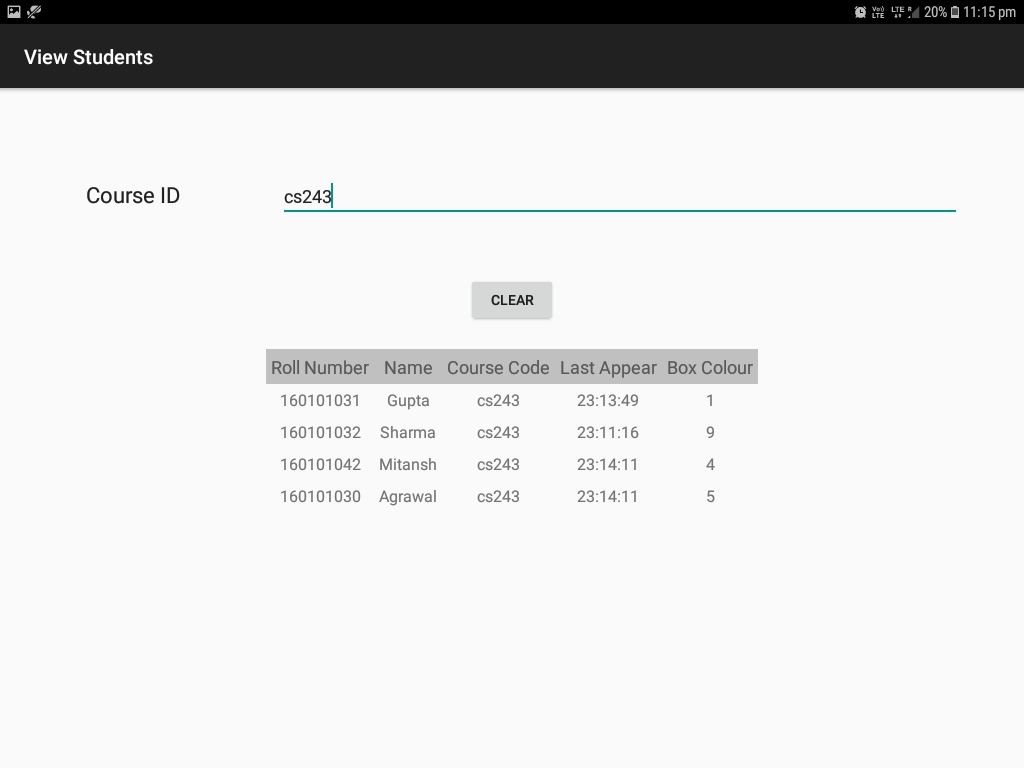
\includegraphics[width=0.7\textwidth, keepaspectratio]{camstate.jpg}
\end{figure}
\begin{figure}[H]
\centering
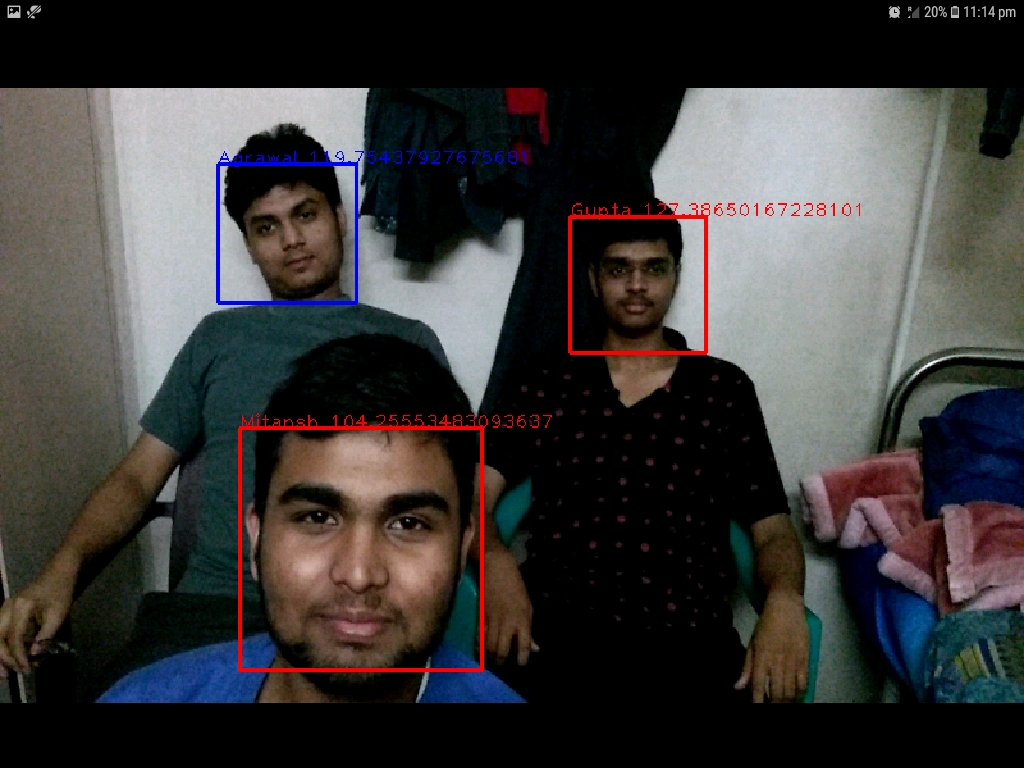
\includegraphics[width=0.7\textwidth, keepaspectratio]{cam3stud.jpg}
\end{figure}
\textbf{Output}: Displays person recognised with corresponding bounding box.We get our desired output.

\item \textbf{Input}: State of student $>$ 8\\
\textbf{Expected Output}: Bounding box color: green
\begin{figure}[H]
\centering
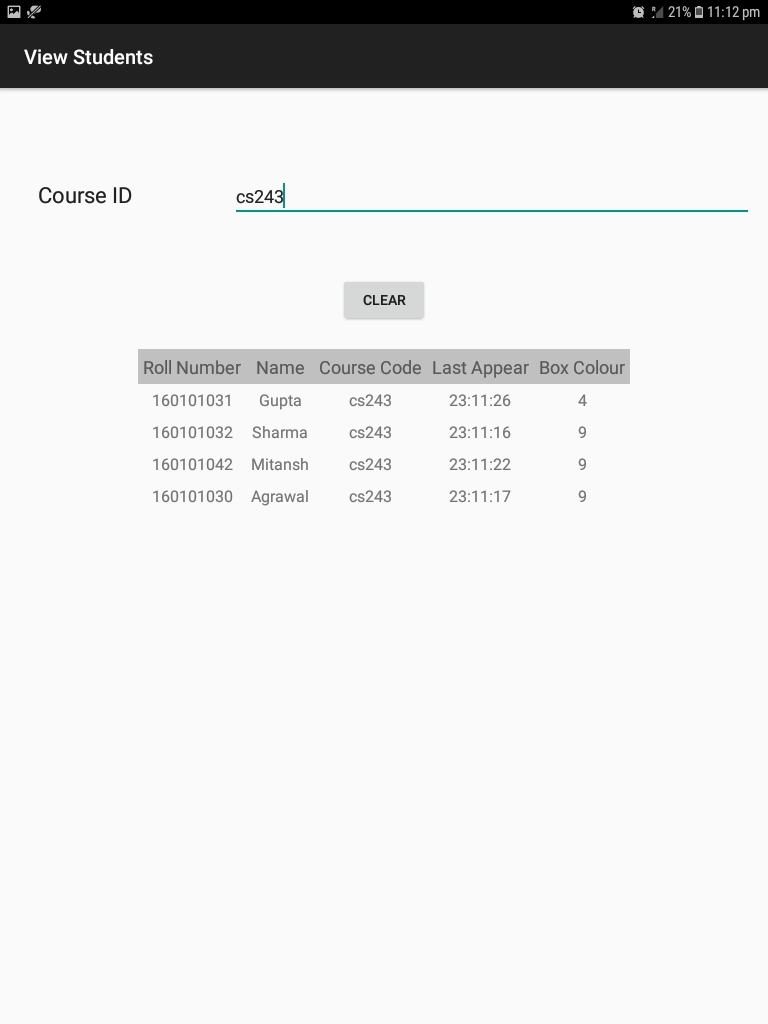
\includegraphics[width=0.42\textwidth, keepaspectratio]{camgr.jpg}
\end{figure}
\begin{figure}[H]
\centering
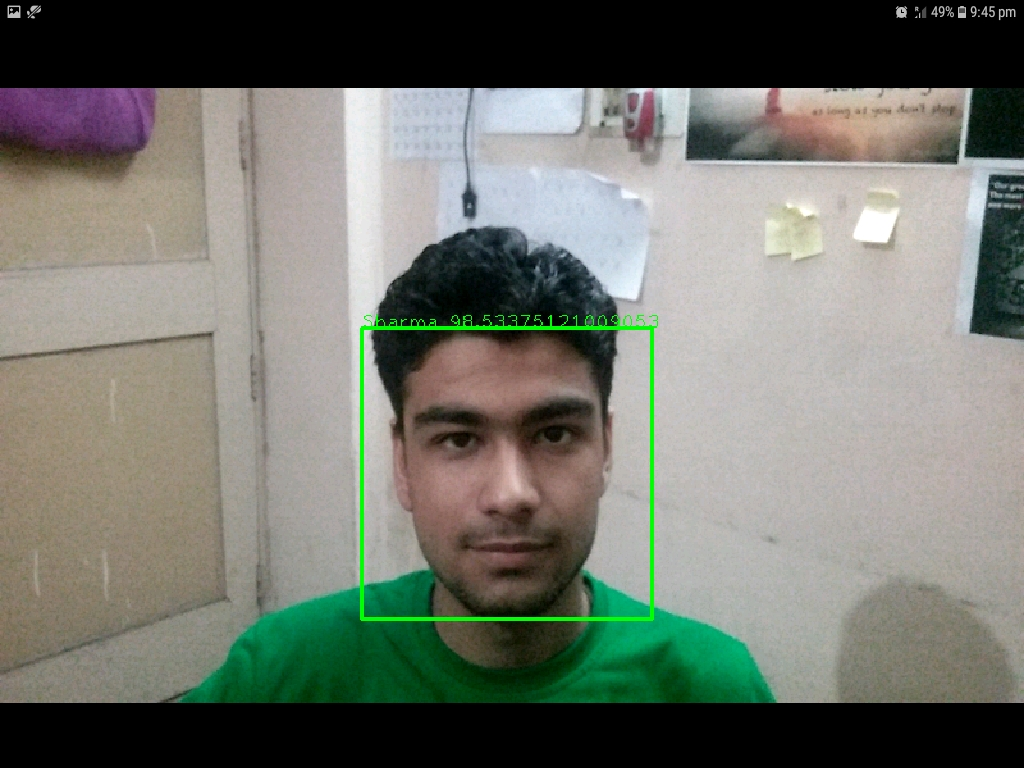
\includegraphics[width=0.7\textwidth, keepaspectratio]{camgrdone.jpg}
\end{figure}
\textbf{Output}: Displays person recognised with corresponding bounding box.We get our desired output.

\item \textbf{Input}: More than one known students(1 to 5) are standing\\
\textbf{Expected Output}: Students should be correctly identified.
\begin{figure}[H]
\centering
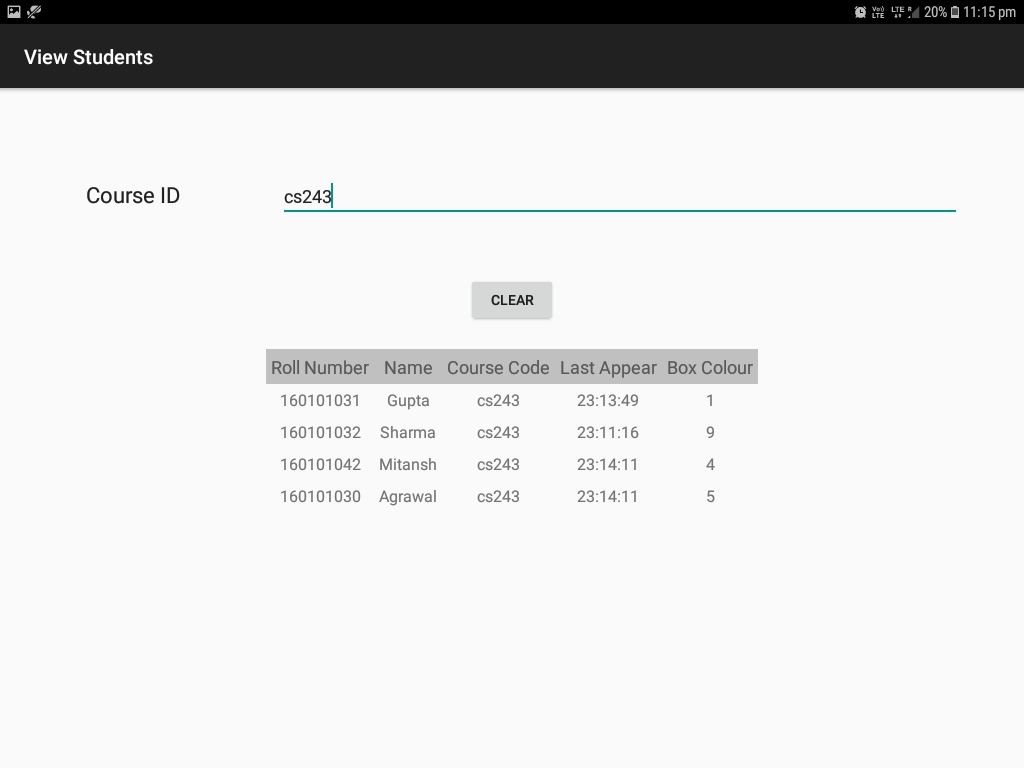
\includegraphics[width=0.7\textwidth, keepaspectratio]{camstate.jpg}
\caption{List of students in class}
\end{figure}
\begin{figure}[H]
\centering
\includegraphics[width=0.7\textwidth, keepaspectratio]{cam3stud.jpg}
\caption{Students identitfied correctly}
\end{figure}
\textbf{Output}: Displays correctly recognised person with corresponding bounding box.We get our desired output.

\newpage
\end{enumerate}
\item[•]\textbf{Boundary Cases}: 
\begin{enumerate}
\item \textbf{Input}: State of student $=$ 5.\\
\textbf{Expected Output}: Bounding box color: blue
\begin{figure}[H]
\centering
\includegraphics[width=0.7\textwidth, keepaspectratio]{camstate.jpg}
\end{figure}
\begin{figure}[H]
\centering
\includegraphics[width=0.7\textwidth, keepaspectratio]{cam3stud.jpg}
\end{figure}
\textbf{Output}: Displays correct bounding box color for state$=$5.We get our desired output.

\item \textbf{Input}: State of student $=$ 8\\
\textbf{Expected Output}: Bounding box color: green
\begin{figure}[H]
\centering
\includegraphics[width=0.42\textwidth, keepaspectratio]{cambon.jpg}
\end{figure}
\begin{figure}[H]
\centering
\includegraphics[width=0.7\textwidth, keepaspectratio]{camboncase.jpg}
\end{figure}
\textbf{Output}: Displays correct bounding box color for state$=$8.We get our desired output.

\item \textbf{Input}: Number of known students $=$ 1\\
\textbf{Expected Output}: Student should be correctly identified.
\begin{figure}[H]
\centering
\includegraphics[width=0.7\textwidth, keepaspectratio]{cam1stud.jpg}
\end{figure}
\textbf{Output}: Displays correctly identified person with its bounding box.We get our desired output.

\item \textbf{Input}: Number of known students $=$ 0\\
\textbf{Expected Output}: Nothing should be shown.
\begin{figure}[H]
\centering
\includegraphics[width=0.7\textwidth, keepaspectratio]{camnostud.jpg}
\end{figure}
\textbf{Output}: Does not display any recognised person name .We get our desired output.

\item \textbf{Input}: Number of unknown students $=$ 1\\
\textbf{Expected Output}: Student should marked with unknown.
\begin{figure}[H]
\centering
\includegraphics[width=0.7\textwidth, keepaspectratio]{camunknown.jpg}
\end{figure}
\textbf{Output}: Recognises the person to be "Mitansh" although he is a unknown student. It may be due to light conditions and face orientation as openCV is very sensitive to these aspects. If any unkwown person comes, it compares with all persons in database and finds nearest possible match.


\end{enumerate}
\end{itemize}
\chapter{White Box Testing}


\section{Module: Sign Up}
\subsection{Funtion: signup()}
\begin{figure}[H]
\centering
\includegraphics[width=\textwidth, keepaspectratio]{signupCode.png}
\caption{Code for signup() function}
\end{figure}

\begin{figure}[H]
\centering
\includegraphics[width=0.16\textwidth, keepaspectratio]{signup.png}
\caption{CFG for signup() function}
\end{figure}
\subsubsection{Calculation of Linearly Independent Paths}
\textbf{Number of Linearly independent paths} = Number of Bounded Regions + 1 = 2
\subsubsection{Linearly Independent Paths}
\begin{enumerate}

\item[•](1-2)-$>$3-$>$(4-6)
\begin{itemize}
\item[]\textbf{Testcase: } validate = False
\item[]\textbf{Expected Output: } Call onSignupFailed() and thus display "signup failed" message.
\item[]\textbf{Observed Output: } Displays "signup failed" message.
\end{itemize}

\item[•](1-2)-$>$3-$>$(7-17)-$>$(18-29)
\begin{itemize}
\item[]\textbf{Testcase: }validate = True
\item[]\textbf{Expected Output: }Call database function to build database, table and insert data.
\item[]\textbf{Observed Output: }Data is inserted according to code.
\end{itemize}

\end{enumerate}

\subsection{Funtion: CheckEmailAlreadyExists()}
\begin{figure}[H]
\centering
\includegraphics[width=\textwidth, keepaspectratio]{checkEmailAlreadyExistsCode.png}
\caption{Code for CheckEmailAlreadyExists() function}
\end{figure}

\begin{figure}[H]
\centering
\includegraphics[width=0.1\textwidth, keepaspectratio]{checkEmailAlreadyExists.png}
\caption{CFG for CheckEmailAlreadyExists() function}
\end{figure}

\newpage


\subsubsection{Calculation of Linearly Independent Paths}
\textbf{Number of Linearly independent paths} = Number of Bounded Regions + 1 = 2
\subsubsection{Linearly Independent Paths}
\begin{enumerate}
\item[•](1-2)-$>$3-$>$(4-6)
\begin{itemize}
\item[]\textbf{Testcase: }ifEmailExists is False(i.e. if email does not exists in database)
\item[]\textbf{Expected Output: }F_RESULT = "Not Found"
\item[]\textbf{Observed Output: }F_RESULT = "Not Found"
\end{itemize}

\item[•](1-2)-$>$3-$>$(7-17)-$>$(18-29)
\begin{itemize}
\item[]\textbf{Testcase: }ifEmailExists is True(i.e. if email exists in database)
\item[]\textbf{Expected Output: }F_RESULT = "Email Found"
\item[]\textbf{Observed Output: }F_RESULT = "Email Found"
\end{itemize}

\end{enumerate}

\subsection{Funtion: CheckFinalResult()}
\begin{figure}[H]
\centering
\includegraphics[width=\textwidth, keepaspectratio]{checkFinalResultCode.png}
\caption{Code for CheckFinalResult() function}
\end{figure}

\begin{figure}[H]
\centering
\includegraphics[width=0.6\textwidth, keepaspectratio]{checkFinalResult.png}
\caption{CFG for checkFinalResult() function}
\end{figure}


\newpage


\subsubsection{Calculation of Linearly Independent Paths}
\textbf{Number of Linearly independent paths} = Number of Bounded Regions + 1 = 3
\subsubsection{Linearly Independent Paths}
\begin{enumerate}
\item[•]1-$>$2-$>$(3-4)-$>$12-$>$13
\begin{itemize}
\item[]\textbf{Testcase: }F_RESULT = "Email Found"
\item[]\textbf{Expected Output: }Toast.text = "Email Already Exists"
\item[]\textbf{Observed Output: }F_RESULT = "Email Already Exists"
\end{itemize}

\item[•]1-$>$2-$>$(5-6)-$>$7-$>$8-$>$11-$>$12-$>$13
\begin{itemize}
\item[]\textbf{Testcase: }F_RESULT = "Not Found" and val = False
\item[]\textbf{Expected Output: }Call onSignupFailed()
\item[]\textbf{Observed Output: }Calls onSignupFailed()
\end{itemize}

\item[•]1-$>$2-$>$(5-6)-$>$7-$>$(9-10)-$>$11-$>$12-$>$13
\begin{itemize}
\item[]\textbf{Testcase: }F_RESULT = "Not Found" and val = False
\item[]\textbf{Expected Output: }Call onSignupSuccess()
\item[]\textbf{Observed Output: }Call onSignupSuccess()
\end{itemize}

\end{enumerate}	

\subsection{Funtion: validate()}
\begin{figure}[H]
\centering
\includegraphics[width=\textwidth, keepaspectratio]{validateSignupCode.png}
\caption{Code for validate() function}
\end{figure}

\begin{figure}[H]
\centering
\includegraphics[width=0.4\textwidth, keepaspectratio]{validateSignup.png}
\caption{CFG for validate() function}
\end{figure}


\newpage


\subsubsection{Calculation of Linearly Independent Paths}
\textbf{Number of Linearly independent paths} = Number of Bounded Regions + 1 = 5
\subsubsection{Linearly Independent Paths}
\begin{enumerate}
\item[•](1-6)-$>$7-$>$(8-9)-$>$13-$>$(16-18)-$>$19-$>$(22-24)-$>$25-$>$(28-30)-$>$31
\begin{itemize}
\item[]\textbf{Testcase: }name = "", email = "a@gmail.com", password="abcde", reEnterPassword="abcde"
\item[]\textbf{Expected Output: }valid = false
\item[]\textbf{Observed Output: }valid = false
\end{itemize}

\item[•](1-6)-$>$7-$>$(10-12)-$>$13-$>$(14-15)-$>$19-$>$(22-24)-$>$25-$>$(28-30)-$>$31
\begin{itemize}
\item[]\textbf{Testcase: }name = "abcde", email = "", password="abcde", reEnterPassword="abcde"
\item[]\textbf{Expected Output: }valid = false
\item[]\textbf{Observed Output: }valid = false
\end{itemize}

\item[•](1-6)-$>$7-$>$(10-12)-$>$13-$>$(16-18)-$>$19-$>$(20-22)-$>$25-$>$(28-30)-$>$31
\begin{itemize}
\item[]\textbf{Testcase: }name = "abcde", email = "a@gmail.com", password="", reEnterPassword="abcde"
\item[]\textbf{Expected Output: }valid = false
\item[]\textbf{Observed Output: }valid = false
\end{itemize}

\item[•](1-6)-$>$7-$>$(10-12)-$>$13-$>$(16-18)-$>$19-$>$(22-24)-$>$25-$>$(26-27)-$>$31
\begin{itemize}
\item[]\textbf{Testcase: }name = "abcde", email = "a@gmail.com", password="abcde", reEnterPassword="abcdefg"
\item[]\textbf{Expected Output: }valid = false
\item[]\textbf{Observed Output: }valid = false
\end{itemize}

\item[•](1-6)-$>$7-$>$(10-12)-$>$13-$>$(16-18)-$>$19-$>$(22-24)-$>$25-$>$(28-30)-$>$31
\begin{itemize}
\item[]\textbf{Testcase: }name="abcde", email="a@gmail.com", password="abcde", reEnterPassword="abcde"
\item[]\textbf{Expected Output: }valid = true
\item[]\textbf{Observed Output: }valid = true
\end{itemize}

\end{enumerate}	

\section{Module: AddStudentRecord}
\subsection{Funtion: AddData()}
\begin{figure}[H]
\centering
\includegraphics[width=\textwidth, keepaspectratio]{addDataCode.png}
\caption{Code for addData() function}
\end{figure}

\begin{figure}[H]
\centering
\includegraphics[width=0.6\textwidth, keepaspectratio]{addData.png}
\caption{CFG for addData() function}
\end{figure}


\newpage


\subsubsection{Calculation of Linearly Independent Paths}
\textbf{Maximum number of Linearly independent paths} = Number of Bounded Regions + 1 = 6
\subsubsection{Linearly Independent Paths}
\begin{enumerate}
\item[•](1-11)-$>$12-$>$(13-17)-$>$21-$>$22-$>$(44-47)
\begin{itemize}
\item[]\textbf{Testcase: }courseID="", name="abc", surname="def", rollID=123
\item[]\textbf{Expected Output: }Toast.text = "Field is Empty"
\item[]\textbf{Observed Output: }Toast.text = "Field is Empty"
\end{itemize}

\item[•](1-11)-$>$12-$>$(13-17)-$>$21-$>$24-$>$(25-26)-$>$29-$>$(30-34)-$>$(44-47)
\begin{itemize}
\item[]\textbf{Testcase: }courseID="cs243", name="abc", surname="def", rollID=123, isInserted=true
\item[]\textbf{Expected Output: }Toast.text = "Data inserted"
\item[]\textbf{Observed Output: }Toast.text = "Data inserted"
\end{itemize}

\item[•](1-11)-$>$12-$>$(13-17)-$>$21-$>$24-$>$(25-26)-$>$29-$>$(35-37)-$>$(44-47)
\begin{itemize}
\item[]\textbf{Testcase: }courseID="cs243", name="abc", surname="def", rollID=123, isInserted=false
\item[]\textbf{Expected Output: }Toast.text = "Data not inserted"
\item[]\textbf{Observed Output: }Toast.text = "Data not inserted"
\end{itemize}

\item[•](1-11)-$>$12-$>$(13-17)-$>$21-$>$24-$>$(38-40)-$>$(44-47)
\begin{itemize}
\item[]\textbf{Testcase: }courseID="cs243", name="abc", surname="def", rollID=123, isInserted=false
\item[]\textbf{Expected Output: }Toast.text = "Data not inserted"
\item[]\textbf{Observed Output: }Toast.text = "Data not inserted"
\end{itemize}

\item[•](1-11)-$>$12-$>$(18-20)-$>$21-$>$(41-43)-$>$(44-47)
\begin{itemize}
\item[]\textbf{Testcase: }courseID="cs243", name="abc", surname="def", rollID="123", isInserted=false
\item[]\textbf{Expected Output: }Toast.text = "Roll Number is not Integer"
\item[]\textbf{Observed Output: }Toast.text = "Roll Number is not Integer"
\end{itemize}

\end{enumerate}	

\section{Module: AddImages}
\subsection{Funtions: onResume(), addimage(), btnTakePhotoClicker.OnClickListener()}
\begin{figure}[H]
\centering
\includegraphics[width=\textwidth, keepaspectratio]{addImagesCode.png}
\end{figure}

\begin{figure}[H]
\centering
\includegraphics[width=0.3\textwidth, keepaspectratio]{addImages.png}
\end{figure}


\newpage


\subsubsection{Calculation of Linearly Independent Paths}
\textbf{Maximum number of Linearly independent paths} = 3
\subsubsection{Linearly Independent Paths}
\begin{enumerate}
\item[•](2-3)-$>$4-$>$(5)-$>$(24-25)-$>$(30-36)-$>$(27-28)-$>$9-$>$22
\begin{itemize}
\item[]\textbf{Testcase: }tempCounter = 5
\item[]\textbf{Expected Output: }Call addImage()
\item[]\textbf{Observed Output: }Calls addImage()
\end{itemize}

\item[•](2-3)-$>$4-$>$(6-8)-$>$9-$>$(10-21)-$>$22
\begin{itemize}
\item[]\textbf{Testcase: }tempCounter = 15
\item[]\textbf{Expected Output: }Set button.text = "Return to Main Menu"
\item[]\textbf{Observed Output: }Set button.text = "Return to Main Menu"
\end{itemize}

\end{enumerate}	

\section{Module: DeleteStudent}
\subsection{Funtion: deleteStudent()}
\begin{figure}[H]
\centering
\includegraphics[width=\textwidth, keepaspectratio]{deleteStudentcode.png}
\caption{Code for deleteStudent() function}
\end{figure}

\begin{figure}[H]
\centering
\includegraphics[width=0.3\textwidth, keepaspectratio]{deleteStudent.png}
\caption{CFG for deleteStudent() function}
\end{figure}



\subsubsection{Calculation of Linearly Independent Paths}
\textbf{Maximum number of Linearly independent paths} = Number of Bounded Regions + 1 = 6
\subsubsection{Linearly Independent Paths}
\begin{enumerate}
\item[•](1-8)-$>$9-$>$(10-11)-$>$(12-14)-$>$18-$>$19-$>$(31-34)
\begin{itemize}
\item[]\textbf{Testcase: }roll_number = ""
\item[]\textbf{Expected Output: }Toast.text = "Field(s) is Empty"
\item[]\textbf{Observed Output: }Toast.text = "Field(s) is Empty"
\end{itemize}

\item[•](1-8)-$>$9-$>$(10-11)-$>$(12-14)-$>$18-$>$(20-22)-$>$23-$>$24-$>$(31-34)
\begin{itemize}
\item[]\textbf{Testcase: }roll_number = 160101042
\item[]\textbf{Expected Output: }Toast.text = "Data is Deleted"
\item[]\textbf{Observed Output: }Toast.text = "Data is Deleted"
\end{itemize}

\item[•](1-8)-$>$9-$>$(10-11)-$>$(12-14)-$>$18-$>$(20-22)-$>$23-$>$(25-27)-$>$(31-34)
\begin{itemize}
\item[]\textbf{Testcase: }roll_number = 160101042
\item[]\textbf{Expected Output: }Toast.text = "Roll ID is not present in database"
\item[]\textbf{Observed Output: }Toast.text = "Roll ID is not present in database"
\end{itemize}

\item[•](1-8)-$>$9-$>$(15-17)-$>$18-$>$(28-30)-$>$(31-34)
\begin{itemize}
\item[]\textbf{Testcase: }roll_number = "abcde"
\item[]\textbf{Expected Output: }Toast.text = "Entered Roll ID not integer"
\item[]\textbf{Observed Output: }Toast.text = "Entered Roll ID not integer"
\end{itemize}

\item[•](1-8)-$>$9-$>$(10-11)-$>$18-$>$(28-30)-$>$(31-34)
\begin{itemize}
\item[]\textbf{Testcase: }roll_number = "abcde"
\item[]\textbf{Expected Output: }Toast.text = "Entered Roll ID not integer"
\item[]\textbf{Observed Output: }Toast.text = "Entered Roll ID not integer"
\end{itemize}

\end{enumerate}	

\section{Module: EditStudent}
\subsection{Funtion: UpdateData()}
\begin{figure}[H]
\centering
\includegraphics[width=\textwidth, keepaspectratio]{updateDataCode.png}
\caption{Code for UpdateData() function}
\end{figure}

\begin{figure}[H]
\centering
\includegraphics[width=0.3\textwidth, keepaspectratio]{updateData.png}
\caption{CFG for UpdateData() function}
\end{figure}



\subsubsection{Calculation of Linearly Independent Paths}
\textbf{Maximum number of Linearly independent paths} = Number of Bounded Regions + 1 = 4
\subsubsection{Linearly Independent Paths}
\begin{enumerate}
\item[•](1-7)-$>$8-$>$(9-10)-$>$(16-18)-$>$19-$>$20-$>$(20-28)
\begin{itemize}
\item[]\textbf{Testcase: }roll_number=160101085
\item[]\textbf{Expected Output: }Toast.text = "Data Updated"
\item[]\textbf{Observed Output: }Toast.text = "Data Updated"
\end{itemize}

\item[•](1-7)-$>$8-$>$(9-10)-$>$(16-18)-$>$19-$>$(21-23)-$>$(26-28)
\begin{itemize}
\item[]\textbf{Testcase: }roll_number=123
\item[]\textbf{Expected Output: }Toast.text = "Data not Updated"
\item[]\textbf{Observed Output: }Toast.text = "Data not Updated"
\end{itemize}

\item[•](1-7)-$>$8-$>$(11-14)-$>$15-$>$(24-25)-$>$(26-28)
\begin{itemize}
\item[]\textbf{Testcase: }roll_number="abcde"
\item[]\textbf{Expected Output: }Toast.text = "Rol Number is not integer"
\item[]\textbf{Observed Output: }Toast.text = "Rol Number is not integer"
\end{itemize}

\end{enumerate}	

\subsection{Funtion: UpdateImages()}
\begin{figure}[H]
\centering
\includegraphics[width=\textwidth, keepaspectratio]{updateImagesCode.png}
\caption{Code for UpdateImages() function}
\end{figure}

\begin{figure}[H]
\centering
\includegraphics[width=0.4\textwidth, keepaspectratio]{updateImages.png}
\caption{CFG for UpdateImages() function}
\end{figure}


\subsubsection{Calculation of Linearly Independent Paths}
\textbf{Maximum number of Linearly independent paths} = Number of Bounded Regions + 1 = 6
\subsubsection{Linearly Independent Paths}
\begin{enumerate}
\item[•](1-11)-$>$12-$>$(13-15)-$>$20-$>$(42-45)
\begin{itemize}
\item[]\textbf{Testcase: }roll_number=""
\item[]\textbf{Expected Output: }Toast.text = "Field(s) is empty"
\item[]\textbf{Observed Output: }Toast.text = "Field(s) is empty"
\end{itemize}

\item[•](1-11)-$>$12-$>$(13-15)-$>$19-$>$21-$>$22-$>$23-$>$24-$>$(25-32)-$>$(42-45)
\begin{itemize}
\item[]\textbf{Testcase: }roll_number=160101032
\item[]\textbf{Expected Output: }Toast.text = "Images Deleted" and prompt to click new Images
\item[]\textbf{Observed Output: }Toast.text = "Images Deleted" and prompt to click new Images
\end{itemize}

\item[•](1-11)-$>$12-$>$(13-15)-$>$19-$>$21-$>$22-$>$24-$>$23-$>$(33-35)-$>$(42-45)
\begin{itemize}
\item[]\textbf{Testcase: }roll_number=160101026
\item[]\textbf{Expected Output: }Toast.text="Roll ID with given corse not in database"
\item[]\textbf{Observed Output: }Toast.text="Roll ID with given corse not in database"
\end{itemize}

\item[•](1-11)-$>$12-$>$(13-15)-$>$20-$>$(36-38)-$>$(42-45)
\begin{itemize}
\item[]\textbf{Testcase: }roll_number=160101031
\item[]\textbf{Expected Output: }Toast.text="Roll ID with given course not present"
\item[]\textbf{Observed Output: }Toast.text="Roll ID with given course not present"
\end{itemize}


\item[•](1-11)-$>$12-$>$(13-15)-$>$20-$>$(36-38)-$>$(42-45)
\begin{itemize}
\item[]\textbf{Testcase: }roll_number="abcde"
\item[]\textbf{Expected Output: }Toast.text="Enteres Roll ID is not integer"
\item[]\textbf{Observed Output: }Toast.text="Roll ID with given course not present"
\end{itemize}

\end{enumerate}	

\section{Module: Login}
\subsection{Funtion: login()}
\begin{figure}[H]
\centering
\includegraphics[width=\textwidth, keepaspectratio]{loginCode.png}
\caption{Code for login() function}
\end{figure}

\begin{figure}[H]
\centering
\includegraphics[width=0.1\textwidth, keepaspectratio]{login.png}
\caption{CFG for login() function}
\end{figure}


\newpage


\subsubsection{Calculation of Linearly Independent Paths}
\textbf{Number of Linearly independent paths} = Number of Bounded Regions + 1 = 3
\subsubsection{Linearly Independent Paths}
\begin{enumerate}
\item[•]1-$>$2-$>$(6-14)-$>$15-$>$(26-27)-$>$(28-39)-$>$40
\begin{itemize}
\item[]\textbf{Testcase: }validate = false
\item[]\textbf{Expected Output: }Call onLoginFailed and set toast.text = "Login Failed"
\item[]\textbf{Observed Output: }Call onLoginFailed and set toast.text = "Login Failed"
\end{itemize}

\item[•]1-$>$12-$>$(3-5)-$>$40
\begin{itemize}
\item[]\textbf{Testcase: }validate = true, result.getCount() = 0
\item[]\textbf{Expected Output: }Call onLoginFailed and set toast.text = "Login Failed"
\item[]\textbf{Observed Output: }Call onLoginFailed and set toast.text = "Login Failed"
\end{itemize}

\item[•]1-$>$2-$>$(6-14)-$>$15-$>$(16-25)-$>$40
\begin{itemize}
\item[]\textbf{Testcase: }validate = true, result.getCount() = 0
\item[]\textbf{Expected Output: }Call onLoginSuccess and set toast.text = "Login Successful"
\item[]\textbf{Observed Output: }Call onLoginSuccess and set toast.text = "Login Successful"
\end{itemize}
\end{enumerate}	

\subsection{Funtion: validate()}
\begin{figure}[H]
\centering
\includegraphics[width=\textwidth, keepaspectratio]{validateLoginCode.png}
\caption{Code for Validate() function}
\end{figure}

\begin{figure}[H]
\centering
\includegraphics[width=0.3\textwidth, keepaspectratio]{validateLogin.png}
\caption{CFG for Validate() function}
\end{figure}


\subsubsection{Calculation of Linearly Independent Paths}
\textbf{Number of Linearly independent paths} = Number of Bounded Regions + 1 = 6
\subsubsection{Linearly Independent Paths}
\begin{enumerate}
\item[•](1-4)-$>$5-$>$(6-7)-$>$11-$>$(12-13)-$>$17
\begin{itemize}
\item[]\textbf{Testcase: }email="a@gmail.com", password=12345
\item[]\textbf{Expected Output: }valid=true
\item[]\textbf{Observed Output: }valid=true
\end{itemize}


\item[•](1-4)-$>$5-$>$(8-10)-$>$11-$>$(12-13)-$>$17
\begin{itemize}
\item[]\textbf{Testcase: }email="", password=12345
\item[]\textbf{Expected Output: }_emailText.error = "enter a valid email address"
\item[]\textbf{Observed Output: }_emailText.error = "enter a valid email address"
\end{itemize}

\item[•](1-4)-$>$5-$>$(6-7)-$>$11-$>$(14-16)-$>$17
\begin{itemize}
\item[]\textbf{Testcase: }email="a@gmail.com", password=""
\item[]\textbf{Expected Output: }passwordText.error = "between 4 and 10 character"
\item[]\textbf{Observed Output: }passwordText.error = "between 4 and 10 character"
\end{itemize}

\end{enumerate}	


\chapter{Conclusion}
The black-box testing and white-box testing were quite successful. 
In black-box testing it was found that app was able to identify people with a good success rate(85\%). It was not able to label unknown people with label "unknown". Almost all the exception handling was found to be handled.
White-box testing was done using path coverage. All the statements of almost all the functions were found to be covered in some test case. Expected output matched with observed one in all cases.

\end{document}
